\documentclass[]{dukedissertation}
%\documentclass[economy,twoside,bind]{dukedissertation}
% Use the second for a single-spaced copy suitable for duplex printing
% and binding.

% Other useful options (there are more options documented in Chapter 2):
%  * draft -- don't actually include images, print a black bar on overful
%             hboxes
%  * MS    -- Format for a Master's Thesis.  No UMI abstract page, some 
%             textual changes to title page.  


% Useful packages for dissertation writing:
\usepackage{amsmath, amssymb, amsfonts, amsthm}
\usepackage{graphicx}
\usepackage{natbib}
\usepackage{color}
\usepackage{bm}
\usepackage{subfigure}
\usepackage{graphicx}
\usepackage{mathabx}
\usepackage{multirow}
\usepackage{setspace}
% \usepackage{cite}  % If you include this, hyperlink cites will
                     % break.  It's nice to use this package if your bibstyle
							% sorts entries by order-of-use, rather than
							% alphabetically (as plain does).
							
%Theorem, Lemma, etc. environments
\newtheorem{theorem}{Theorem}%[section]
\newtheorem{lemma}[theorem]{Lemma}
\newtheorem{proposition}[theorem]{Proposition}
\newtheorem{corollary}[theorem]{Corollary}
\newtheorem{result}[theorem]{Result}

% Personal commands and abbreviations.
%Define and personal commands here

%Graphics Path to find your pictures
\graphicspath{{./Pictures/}{../figure/}}


%-----------------------------------------------------------------------------%
% PREAMBLE 
%-----------------------------------------------------------------------------%
\author{Anh Le}
\title{Two-Sided Matching Model}
\supervisora{Michael Ward}
\supervisorb{Eddy Malesky}
\department{Department of Political Science} % Appears as Department of \department
% Declare dissertation subject used on UMI abstract page.  List of
% categories: http://dissertations.umi.com/duke/subject_categories.html
%\subject{[Your Subject Here]}

\date{2018} % Anything but the year is ignored.

% Copyright text.  If undefined, default is 'All rights reserved'
% (Example sets the text to a hyperlinked Creative Commons Licence)
\copyrighttext{ All rights reserved except the rights granted by the\\
   \href{http://creativecommons.org/licenses/by-nc/3.0/us/}
        {Creative Commons Attribution-Noncommercial Licence}
}

% Committee Members other than supervisor.  No more than five beyond the
% supervisor allowed.
\member{Daniel Stegmueller}
\member{Peter Hoff}
%-----------------------------------------------------------------------------%


%-----------------------------------------------------------------------------%
% HYPERREF: plain black hypertext references for ref's and cite's.
%-----------------------------------------------------------------------------%
\usepackage[pdftex, pdfusetitle, plainpages=false, 
				letterpaper, bookmarks, bookmarksnumbered,
				colorlinks, linkcolor=black, citecolor=black,
	         filecolor=black, urlcolor=black]
				{hyperref}

\begin{document}

%-----------------------------------------------------------------------------%
% TITLE PAGE -- provides UMI abstract title page & copyright if appropriate
%-----------------------------------------------------------------------------%
\maketitle

%-----------------------------------------------------------------------------%
% ABSTRACT -- included file should start with '\abstract'.
%-----------------------------------------------------------------------------%
% \abstract

While a Foreign Direct Investment (FDI) project can only materialize with the consent of both the multinational corporation (MNC) and the host country, the literature on FDI has focused only on the preference of MNCs. Through various case studies, I show that countries have varied and strategic preference, playing a substantial role in determining where FDI locates. Failing to recognize this two-sided matching nature of the FDI market, existing models of FDI produce wrong estimates of MNCs' preference. I introduce the two-sided matching model, investigate properties of the model, and apply it to study Japanese FDI in Southeast Asia. I show how to estimate the preference of both MNCs and countries for one another, modeling the two-sided matching process behind FDI location that scholars have always known but never been able to study quantitatively. With this model, scholars have a better understanding of what drives FDI location and policy makers can simulate FDI movement under hypothetical policy changes.}

%-----------------------------------------------------------------------------%
% DEDICATION -- OPTIONAL.  Put the text inside the braces.
%               (Long 'dedications' probably belong in the acknowledgements)
%-----------------------------------------------------------------------------%
%\dedication{If you want to dedicate your thesis to anyone do so here}

%-----------------------------------------------------------------------------%
% FRONTMATTER -- ToC is required, LoT and LoF are required if you have any
% tables or figures, respectively. List of Abbreviations and Symbols is 
% optional.
%-----------------------------------------------------------------------------%
\tableofcontents % Automatically generated
\listoftables	% If you have any tables, automatically generated
\listoffigures	% If you have any figures, automatically generated
\abbreviations

% You can put here what you like, but here's an example
%Note the use of starred section commands here to produce proper division
%headers without bad '0.1' numbers or entries into the Table of Contents.
%Using the {\verb \begin{symbollist} } environment ensures that entries are
%properly spaced.

% \section*{Symbols}

% Put general notes about symbol usage in text here.  Notice this text is
% double-spaced, as required.

% \begin{symbollist}
% 	\item[$\mathbb{X}$] A blackboard bold $X$.  Neat.
% 	% Optional item argument makes the symbol/abbr
% 	\item[$\mathcal{X}$] A caligraphic $X$.  Neat.
% 	\item[$\mathfrak{X}$] A fraktur $X$.  Neat.
% 	\item[$\mathbf{X}$] A boldface $X$.
% 	\item[$\mathsf{X}$] A sans-serif $X$. Bad notation.
% 	\item[$\mathrm{X}$] A roman $X$.
% \end{symbollist}

\section*{Abbreviations}

\begin{symbollist}
  \item[AmCham] American Chamber of Commerce
  \item[ASEAN] Association of Southeast Asian nations
  \item[DGP] Data generating process
  \item[EM] Expectation maximization
	\item[FDI] Foreign direct investment
  \item[IPA] Investment promotion agency
  \item[IPE] International political economy
  \item[LDA] Latent Dirichlet allocation
	\item[MCMC] Markov chain Monte Carlo
  \item[MH] Metropolis-Hastings
	\item[MLE] Maximum likelihood estimation
  \item[MNC] Multinational corporation
  \item[MVN] Multivariate normal
  \item[SOE] State-owned enterprise
  \item[UNCTAD] United Nations Conference on Trade and Development
\end{symbollist}
} % List of Abbreviations. Start file with '\abbreviations'

%-----------------------------------------------------------------------------%
% ACKNOWLEDGEMENTS -- included file should start with '\acknowledgements'
%-----------------------------------------------------------------------------%
%\acknowledgements

I would like to thank my two advisors, Professor Edmund Malesky and Professor
Michael Ward. Professor Malesky's work on foreign direct investment and the
political economy of Vietnam was a big inspiration and \textit{the} reason for my
pursuing a PhD (and choosing Duke!) in the first place. He has taught me many
lessons in designing research, communicating results, and, most importantly,
being a good person. Professor Ward's approach to empirical work was an
eye-opener, pushing me to grow in ways I could not envision before. He nurtured
Ward lab, a community of smart and supportive people that I benefit from
tremendously even to this day. I used to tell every prospective student about
the Ward lab, and I really wish I still could.

I also benefited tremendously from the advice of Professor Peter Hoff and Professor Daniel Stegmueller. Without your kind and patient help, I would not have been able to develop and implement the statistical model for this dissertation. Professor Hoff's ``A First Course in Bayesian Statistical Methods'' is worth its weight in gold.

My thanks also to Professor Michael Newton for discussing two-sided matching model with me out of nothing but generosity, Professor John Allen Logan for sharing his US labor data, and Professor Andrew Delios for sharing his Japanese foreign direct investment data.

Finally, I would like to thank my wife, Huyen Le, for being there. (She did a lot more, but being there was already enough.)

%%% Local Variables:
%%% mode: latex
%%% TeX-master: "../AnhLe_dissertation.tex"
%%% End:}

%==============================================================================
%-----------------------------------------------------------------------------%
%
% MAIN BODY OF PAPER
%
%
%-----------------------------------------------------------------------------%
\chapter{Introduction}
\label{chap:introduction}

The global flow of Foreign Direct Investment (FDI) has risen from almost nothing
in the 1970s to over \$2.3 trillion dollars in 2016, becoming an important
source of global capital (Figure~\ref{fig:globalfdi}). For developing countries
especially, capital from multinational corporations (MNCs) is robust to global
economic downturns, prompting major international organizations to endorse FDI
as a key factor to economic development and poverty reduction
\citep{Mallampally1999, WorldEconomicForum2013}.\footnote{Indeed, while FDI into
  developed economies dropped almost 50\% during the 2000 recession and the 2008
  financial crisis, FDI into developing countries only experienced a plateau or
  a small reduction. More recently, as global FDI flow slipped in 2016 and 2017,
  FDI into developing countries still remained stable \citep{UNCTAD2018}.} Within the scholarly
field of International Political Economy (IPE), much of the literature starts
with the view that countries will always seek FDI for its various benefits
\citep{Jensen2008b}. Works in IPE tend to focus on \textit{how} countries can
attract FDI, and do not question \textit{whether} they want to do so
\citep{Jensen2003, Li2003, Li2006, Ahlquist2006}.\footnote{Two recent exceptions
  are \citet{Pinto2013, Pandya2016}, who are the first to examine variation in
  countries' demand for FDI.}

\begin{figure}[tbp]
  \centering
  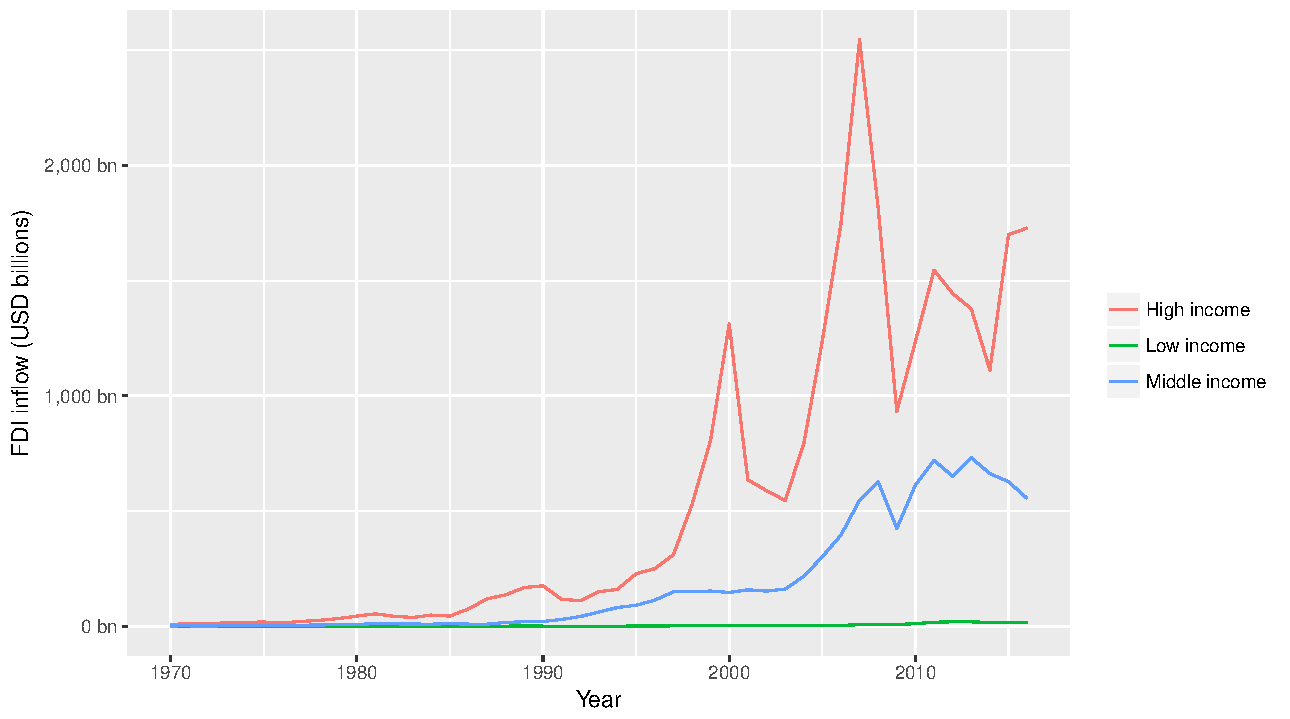
\includegraphics[width=0.8\textwidth,keepaspectratio]{../figure/global_fdi}
  \caption[FDI global inflow, 1970-2006.]{FDI global inflow, 1970-2006. The last
    four decades witness the growth of FDI into the most important source of
    global capital. Source: World Bank's World Development Indicators.}
  \label{fig:globalfdi}
\end{figure}

At first glance, the benefits of FDI seem obvious. FDI brings capital, create
jobs, contribute tax revenue, and promise technological spillover to the local
economy. Consider the impact of a high-tech facility by Intel on Vietnam's
economy. In 2006, Intel announced Saigon Hi-tech Park in Ho Chi Minh City,
Vietnam as the site for its largest chip testing and assembly in the world.
Starting from the initial plan of a US\$300 million facility, Intel decided
eight months later to increase the investment to US\$1 billion dollar, making up
almost 10\% of Vietnam's registered FDI in 2006. In 2016, Intel Products Vietnam
(IPV) employed 4000 workers at full capacity, exported US\$3.45 billion worth of
goods (18.2\% of Vietnam's electronics export), and contributes more than
US\$100 million to Vietnam's GDP in tax payment, salary, and profit. More
importantly, IPV also helped Vietnam address the skill shortage in engineering
and management. In the beginning, IPV hired workers earlier and trained them at
other Intel facilities in Asia. In the longer term, IPV developed an engineering
education program in partnership with Arizona State University and local
universities, training thousands of young Vietnamese engineers and giving them a
job. As a result, IPV's workers are vastly more productive: while IPV's
workforce only constituted 5\% of all workers at the Saigon Hi-tech Park, its
export value amounted to 72\%. Finally, Intel's decision to choose Ho Chi Minh
City over other candidate sites, including Chennai (India), Bangkok (Thailand),
and Dalian (China), was a significant marketing boost to Vietnam's image as a
destination capable of high-tech manufacturing. Following Intel, many other MNCs
opened high-tech facilities in Vietnam, including Samsung's three factories (in
2009, 2013, and 2014), Nokia/Microsoft (2012), and LG (2013) \citep{Dinh2016,
  UNCTAD2008}.

From a theoretical perspective, \citet{Findlay1978} argues that FDI plays a key
role in economic growth by upgrading the local economy's technological capability. As
well-known from neoclassical growth theory, diminishing returns to capital will
at one point stop capital from accumulating further, preventing long-run
economic growth from being driven by capital accumulation alone
\citep{Solow1956}. FDI can counteract this dynamic by helping local workers and
suppliers upgrade their productivity, either via training or demonstration.
In other words, technological spillover from FDI shifts the domestic factor-price
frontier to the right, resulting in a continually increasing capital stock and
sustained economic growth.

However, despite the theoretical arguments and shining examples such as Intel in
Vietnam, cross-country studies shows that
not all FDI are the same and that its effects are highly conditional. For
example, there is no conclusive evidence of FDI inflow having a positive effect on
growth \citep{Nair-Reichert2001, Carkovic2002} or poverty reduction
\citep{Guerra2009}. This puzzle opens a substantial literature on how the
growth-enhancing and spillover effect of FDI is conditional on the absorptive
capacity of the host economies, i.e. its level of human capital, technological
sophistication, and financial market development \citep{Durham2004,
  Nunnenkamp2004, Fu2008, Willem2004}. In addition, while the capital brought
and jobs created by FDI may be unconditionally good for the overall economy, its
distributional effects cut across constituencies in the host economy, creating
political cleavage across both sectoral and geographical divides
\citep{Chintrakarn2012, Goldberg2007, Nunnenkamp2007}.

Given the evidence on the conditional effect of FDI, it is no longer tenable to
assume that countries' preference for FDI is homogeneous. By holding this
assumption, we neglect the role of the state in shaping global capital flow,
falling prey to the discredited ``race to the bottom'' thesis of globalization
\citep{Mosley2005}. Arguably, examining countries' preference for FDI should be
of more interest to political scientists than the current focus on determinants
of MNCs' location, which often amounts to adding a political variable to an
existing economic model of FDI flow. In addition, even if we only care about
MNCs' preference, to get an accurate estimate we must still take into account
countries' preference. For example, consider the received wisdom that
democracies receive more FDI \citep{Jensen2008a}. Without controlling for
countries' preferences, it is difficult to interpret this finding as democracies
actively pursuing MNCs or as MNCs finding democracies attractive.

\section{Goal of the research}

My research aims to estimate the preference of countries and MNCs for each
other. I develop an empirical strategy that takes into account the two-sided
nature of the FDI market, i.e. a subsidiary can only materialize if both the MNC
and the host government agree. Recognizing that this two-sided matching dynamics
can also be found in the labor or the marriage markets, I adapt the statistical
models first developed in Sociology for labor and marriage markets and apply
them to the study of FDI \citep{Logan1996, Logan2008}.

In doing so, I simultaneously address three long-standing issues in the FDI
literature. First, I ``bring the state back in,'' filling the gap in the literature on the
variation of countries' preference for FDI.\footnote{\citet{Evans1985}'s
book argues that states are weighty actors with their own capabilities and
initiatives rather than an arena for societal and interest groups to negotiate
for their share. Here, I argue that states are weighty actors with their own
preferences rather than goods that MNCs pick and choose.} Two notable exceptions are
\citet{Pinto2013} and \citet{Pandya2016}, whose pioneering works propose
partisan politics and regime types as factors shaping preferences for FDI.
However, while their theories are ground-breaking, the empirical estimation of
countries' preference remains inadequate. In addition, these researchers have
not used their findings to re-estimate the preference of MNCs and disentangle
the ``push'' and ``pull'' factors of FDI flow.\footnote{``Push factors'' refer
  to characteristics of the home country and of the MNC, pushing capital out
  from its origin. ``Pull factors'' refer to the characteristics of the host
  country, pulling capital towards its destination.} Using a two-sided matching
model, I will naturally be able to estimate both sides' preference.

Second, I propose that we need to pay more attention to countries' preference
for different types of FDI. While the IPE literature has largely focused on the
quantity of FDI flow, countries pay much attention to the its type, using
various incentives and restrictions to target certain types of FDI. Indeed, MNCs
come with varying amount of capital, labor demand, and technological
sophistication, all of which have different effects on the host country's
economy. Just as the two-sided matching model can estimate MNCs' utility
function for countries' characteristics (e.g. market size, level of
development), it can also estimate countries' utility function for MNCs'
characteristics (e.g. technological sophistication, export strategy).

Third, while the majority of the literature uses FDI flow data, these data
are accounting constructs created to keep track of countries' balance of payment
and thus map poorly to concepts in Political Science theories. Very often, the
variable of interest in our theories is the scale of MNCs' activities in the
host country, which can be very different from the amount of border-crossing
capital thanks to MNCs' complex financial and tax strategies \citep{Kerner2014}.
Therefore, we would do much better testing our theories with firm-level
operational data. Because the two-sided matching model is a behavioral model in
which each actor's decision is a unit of observation, and we can naturally use
it to analyze firm-level data.

These three issues are related and represent the status quo in the FDI
literature. Data limitation forces scholars to look at country-level aggregate
FDI flow, making it difficult to study countries' preference for FDI types. And
without studying countries' preference, our current models of MNCs' location
choice are also suspect.

In sum, my dissertation benefits the field by using firm-level data to estimate
both firms' and countries' preference for each other's characteristics. In this
two-sided matching model, MNCs and countries evaluate their available options
according to their utility functions, choose the best alternative, culminating
in an MNC's subsidiary located in a host country.

Estimating this model would be straightforward if we observed not only
subsidiaries' locations but also their set of options (called their
``opportunity set'' in the matching literature).\footnote{Discrete choice models
  can be used to estimate the utility function when both the choice and the set
  of options are observed. Indeed, discrete choice models remain the dominant
  empirical approach in the industrial location literature, effectively ignoring
  the fact that not all MNCs have the same set of location options
  \citep{Arauzo-Carod2010}.} Unfortunately, while data on subsidiaries' location
are available, the opportunity set is generally unobserved as researchers cannot
peek into the negotiation process between countries and MNCs. The two-sided
matching model solves this problem by using the Metropolis-Hastings (MH)
algorithm, a Markov chain Monte Carlo (MCMC) approach that repeatedly samples
new opportunity sets and rejects them at an appropriate rate to approximate
their true distribution. In addition, the estimated preference parameters in the
two-sided model have a convenient interpretation as the relative weight of
different variables on MNCs' and countries' utility. This allows us to make
statements such as: ``In evaluating MNCs, China values a 2\% increase in the
firm's capital as much as a 1\% increase in labor demand.''

\section{Roadmap}

In the rest of this introductory chapter, I review in-depth the three issues in
the literature of FDI's political determinants, outlining the current attempts
to address them and how my approach can contribute to the solution.

In Chapter~\ref{chap:model}, I describe the two-sided matching model, including
both its game-theoretic origin and its statistical estimation.
Chapter~\ref{chap:simulation} uses simulations to demonstrate the correctness of
the model and explore its characteristics. Chapter~\ref{chap:labor} applies the
model on US labor market data, the original domain of the two-sided matching
approach, in order to compare with and expand upon previous results.
Chapter~\ref{chap:FDI} brings us back to the study of FDI, applying the model on
firm-level data of Japanese MNCs in East and Southeast Asia.
Chapter~\ref{chap:conclusion} concludes and explores potential applications of
the two-sided matching model in other areas of Political Science.

\section{Three issues in the FDI literature}
\label{sec:literature_issues}

\subsection{Estimating countries' demand for FDI}

The IPE literature on the political determinants of FDI has overwhelmingly
focused on what MNCs demand from countries, not what countries demand from MNCs.
In this literature, politics matters, but only in terms of what
political factors make countries attractive to MNCs. As Jensen states in
the introduction of \textit{Nation-states and the multinational corporation}:

\begin{quote}
  Which government policies prove beneficial to multinational corporations?
Which political institutions provide multinational corporations with credible
commitments to these market-friendly policies? These emerge as the central
questions of this book.
\end{quote}

Other scholars share the same line of inquiry \citep{Ahlquist2006, Busse2007,
  Buthe2008, Li2003}. In their theoretical argument, the central dynamics of the
negotiation between countries and MNCs is that FDI is mobile before MNCs make
the investment on the ground but immobile after. Since the cost of relocation is
higher the more investment MNCs commit, the original bargain between the host
country and the MNC become increasingly obsolete as the host country can alter
the original bargain at the expense of the MNC, knowing that relocating would
cost the MNC dearly. Therefore, certain political
institutions, such as democracy, veto players, and federalism, increase FDI
inflow because they can credibly commit not to change their policies \textit{ex
  post}, and are thus
attractive to MNCs.

Cost of doing business arguments. 

In theorizing FDI inflow largely as a function of MNCs' preference, the FDI
literature implicitly assumes that countries are eager to receive as much FDI as
possible. The two common empirical approaches in the literature expose this
assumption. In the first approach, researchers build a regression model with FDI
inflow as the dependent variable and a political factor as the independent
variable of interest. The problem with this model is that it is impossible to
interpret the political factor as an attraction to MNC or as a motivator of
countries' demand for FDI. Consider \citet{Jensen2005}'s finding that federalism
is positively associated with FDI inflow. The authors interpret this correlation
as federalism constraining the whim of the central government, increasing policy
stabilities, and thus making the country attractive to MNCs. However, the
alternative explanation is that local governments in a decentralized system
compete more intensely for FDI, driving up the FDI inflow. For example, As China
decentralized in the late 1980s and early 1990s, local governments gained the
authority to approve foreign investment up to a certain size, thus able to court
MNCs without asking the central government for permission.\footnote{Similar to
  China's broader economic reform, decentralization in China's FDI policies
  happened incrementally. In 1979, China first allowed FDI in four Special
  Economic Zones, i.e. Shenzhen, Zhuhai, Shantou (near Hong Kong), and Xiamen
  (near Taiwan). As the economic benefits of FDI became clear, provinces started
  clamoring for the ability to attract FDI themselves. Therefore, in 1984, China
  allowed 14 coastal cities to approve FDI projects themselves, and in the early
  1990s, allowed inland regions to do the same. \citet{Gallagher2002, Shirk1993}
  discuss how the coalition for decentralization expanded over this period, and
  \citet{Coase2012} provides a historical account of China's economic reform
  more broadly.} In addition, local governments could keep all revenue in excess
of a quota pre-negotiated with the central government, further motivating them
to bring in MNCs as a lucrative source of tax revenue. Having both the authority
and the incentive to attract MNCs, Chinese local governments engaged in an
intense competition for MNCs. For example, while there were only 117 development
zones in 1991, the number exploded to 2700 in 1992, of which only 95 were
initiated by central ministries \citep{Montinola1995}. Far from
\citet{Jensen2005}'s argument, China's federalism did not increase FDI inflow by
producing a static policy environment that MNCs like. On the contrary,
federalism incentivized Chinese local governments to demand FDI, fostering
local policy experiments that were anything but stable.\footnote{A very similar
  account of decentralization causing provincial demand and competition for FDI happened in Vietnam
  as well \citep{Malesky2004c}.}

In the second approach, researchers estimate MNCs' preference using discrete
choice model. The dependent variable is the MNC's choice of a location over all
the others, and the independent variable of interest is a characteristic of the
location \citep{Arauzo-Carod2010}. In discrete choice model, the assumption is
that all locations are available for the MNC to pick and choose, effectively
ruling out the possibility that the host country can decline the MNC's
investment proposal. Such an assumption is unfounded. For example, in 2007, Da Nang, a
central province of Vietnam known for its public governance quality, turned down
\$2.5 billion dollars from
a Taiwanese-Japanese steel factory and a Japanese paper pulp factory for
environmental concern \citep{NLD}. In 2014, even in tough times, when Da Nang's and Vietnam's
FDI inflow was
merely half of the previous year, Da Nang's attitude towards FDI remained
selective, declining a \$200-million Hong Kong textile factory and a 30-hectare Korean dying
facility, showing its  

A historical and comparative examination of FDI policies makes it clear that the
assumption of countries' unequivocal demand for FDI is not true. First,
historically countries are not so open to FDI.

Second, there is substantial variation across countries.

Third, countries are very strategic in their FDI policies, changing it over
time to fit with the political and economic conditions of the countries.


We have made this mistake before. Despite earlier pessimism about countries engaging in a race to the bottom to
attract footloose global capital, empirical evidence shows that countries'
policies still vary substantially \citep{Drezner2001}. While the broader IPE
literature has recognized the variation in countries' trade, welfare,
environmental, and fiscal policies in the face of globalization, we have
surprisingly done less work to explain variation in countries' demand for FDI.
Neglecting countries' demand for FDI is both a theoretical and an empirical gap
in our FDI literature. Theoretically, much of the literature on the political
determinants of FDI only examines how the political factors are assessed by the MNC, assume that countries want as much FDI as possible and the
only problem is that they cannot credibly commit to reduce the uncertainty in
order to attract business. On the empirical side, in using discrete choice model
to model MNCs' location decision, the literature assumes that all MNCs have
access to all locations.

Recognizing this gap in the literature, \citet{Pinto2013} and \citet{Pandya2016}
recently broke ground in this area. Similar to the rich IPE literature in
international trade, these studies argue that countries' demand for FDI varies
according to FDI's distributive effect on their domestic constituencies
\citep{Broz2001, Milner2005a}. In this theoretical framework, labor supports FDI
because foreign firms bring capital that increases the demand for labor and
raises productivity, both of which lead to higher wage. On the other hand,
domestic firms oppose FDI because foreign firms compete for local labor, inputs,
and markets. Both \citet{Pinto2013} and \citet{Pandya2016} formulate their
theories as a variant of this labor-vs-business tension, which surfaces in the
former work as left-vs-right governments, and in the latter as
democratic-vs-authoritarian regimes.

While these pioneering works have enriched our understanding of the relationship
between politics and FDI, their empirical approaches do not satisfactorily
measure countries' demand for FDI, leaving their theoretical arguments untested.

Consider \citet{Pinto2013}'s approach. The author controls for economic and
institutional factors that affect FDI flow into a country, then claims that
what's left in the residual is the country's demand for
FDI.\footnote{Specifically, the estimation of FDI openness involves two steps.
  First, the author runs a gravity model explaining bilateral FDI flows,
  estimating the intercept as the host country-year fixed effect. Second, this
  fixed effect is then regressed on several economic and endowment factors of
  that country-year (i.e. GDP, GDP per capita, average school years, arable
  land). The residual in the second stage is considered the country's ``FDI
  openness'' in that year.} For this approach to be valid, every economic,
institutional, and endowment factors that affect FDI flow has to be controlled
for, leaving only the country's demand in the error term. This claim is much
stronger than the common assumption of exogenous error, which is valid as long
as the omitted factors are uncorrelated with the independent variable of
interest. Framed substantively, since the residual is likely to contain more
than just the country's demand for FDI, if we observe an abnormally high level
of FDI, we do not know whether it is because the country welcomes FDI or because
MNCs find something attractive in the country.\footnote{In addition, this
  approach requires data on bilateral FDI flow, ideally disaggregated by
  sectors. Therefore, this approach is limited to OECD countries only
  \citep{Pinto2008}. During the period the authors study, 1980-2000, OECD
  countries account for 95\% of global FDI outflow and 90\% of inflow. However,
  since then the role of the developed world in global FDI has declined sharply,
  reducing to 60.8\% of outflow and 40.6\% of inflow in 2014
  \citep{UNCTAD2015}.}

In contrast to \citet{Pinto2013}'s statistical approach, \citet{Pandya2014,
  Pandya2016} attempts to find a proxy for countries' demand for FDI. The author
uses the annual US Investment Climate Reports to construct the number of
industries that have foreign ownership restrictions or face investment
screening. The advantages of this measurement are its ease of interpretation and
its availability for many countries. However, two problems remain. First, adding
up the raw count of restricted industries is not appropriate because industries
are not the same. For example, given the reach of the banking sector into all
corners of the economy, a country's opening up its financial industry indicates
much more FDI-friendliness than, say, allowing foreign furniture makers to set
up shops. Since the theoretical argument is driven by FDI's distributive effect,
we must not ignore the varying impact of FDI across sectoral constituencies.

Second, according to the coding rule, an industry is coded as free if there is
no mention of restriction. However, when there is little FDI, US Investment
Climate Report may find it not worth mentioning and does not report the
restrictions. Therefore, ``zero restriction'' in the dataset can either mean
that a country is very closed or very open to FDI. This concern is not
hypothetical. Figure \ref{fig:china_fdi_restriction} shows that, following the
coding of the US Investment Climate Reports, China seemed 100\% open to FDI up
until 1986 when it started imposing restrictions. The reality is the opposite.
Prior to 1986, only limited FDI was allowed as joint-venture in Special Economic
Zones (SEZ). The year of 1986 was, in fact, the first time China allowed any
wholly owned FDI outside of SEZs.

\begin{figure}[tbp] \centering
  \includegraphics[width=0.8\textwidth,keepaspectratio]{china_fdi_restriction}
  \caption[China's FDI ownership restriction.]{China's FDI ownership
    restriction, as coded in \citet{Pandya2010}. Prior to 1986, FDI in China was
    limited to few experimental Special Economic Zones, and thus not mentioned
    in US Investment Reports. The sharp spike in 1988 also does not seem to
    correspond to any actual change in policy, and likely another artifact of
    reporting. (See \citet{Zebregs2002} for a historical overview of China's FDI
    policy.)}
  \label{fig:china_fdi_restriction}
\end{figure}

The two-sided matching model circumvents these thorny measurement issues by
modeling countries' demand for FDI directly. Intuitively, if we observe that a
country welcomes certain firms to invest but not others, we can compare the
characteristics of the invited and the uninvited firms to infer that country's
preference for FDI.

\subsection{Estimating countries' preference for types of FDI}

In addition to estimating countries' demand for FDI, we should also examine
countries' preference for different types of FDI. Indeed, while the Political
Science literature has focused almost exclusively on the quantity of FDI,
treating all FDI as one homogeneous flow of capital, policy makers seem to pay
much more attention to distinguishing its types. Commenting on the role of
International Investment Agreements, \citet{UNCTAD2015} says, ``Today,
increasing the quantity of investment is not enough. What matters is its
quality, i.e. the extent to which investment delivers concrete sustainable
development benefits.'' Governments in developing countries all offer various
forms of tax incentives and fee waivers to attract FDI that invests in a remote
region, brings new technology, or focuses on exporting \citep{Ricupero2000}. For
example, since 2006, China's official FDI policy has been ``quality over
quantity,'' promoting FDI with intense R\&D in high-productivity sectors
\citep{Guangzhou2011}.

Despite the importance of disaggregating FDI by its type, two data limitations
prevent researchers from doing so. First, FDI flow data typically does not
disaggregate into types of FDI. \citet{Alfaro2007} attempt to get around this
problem by using Germany's sectoral skill intensity as the proxy for the FDI
quality from each sector in the OECD. To do so is to assume that 1) Germany's
sectoral variation is the same as everyone else's in the OECD, and 2) there is
little variation in skill intensity within a sector. Both assumptions are
untenable, especially since the authors divide all manufacturing industries into
only two categories: low skill and high skill.

Second, even if we can differentiate types of FDI, it remains an open question
how to estimate countries' preference for them. \citet{Alfaro2007} use
information from IPAs' website and survey response as a proxy for their
countries' preference---if an IPA lists an industry as a ``target industry,''
the authors say that the country wants to attract that type of FDI. While this
approach seems reasonable at first glance,
Figure~\ref{fig:IPA_target_industries} shows that there is little variation in
what IPAs claim to be their target industries. Because investment promotion is
mainly a marketing and aspirational exercise, almost everyone claims that they
target manufacturing, advanced manufacturing, and infrastructure. In addition,
if we use IPAs as a proxy for countries' preferences, we should also model the
selection process in which the countries that decide to establish an IPA may not
be the same as those who do not. Both of these issues are not addressed by
\citet{Alfaro2007}, and we are still in need of a way to estimate countries'
preference for different types of FDI.

\begin{figure}[tbp] \centering
  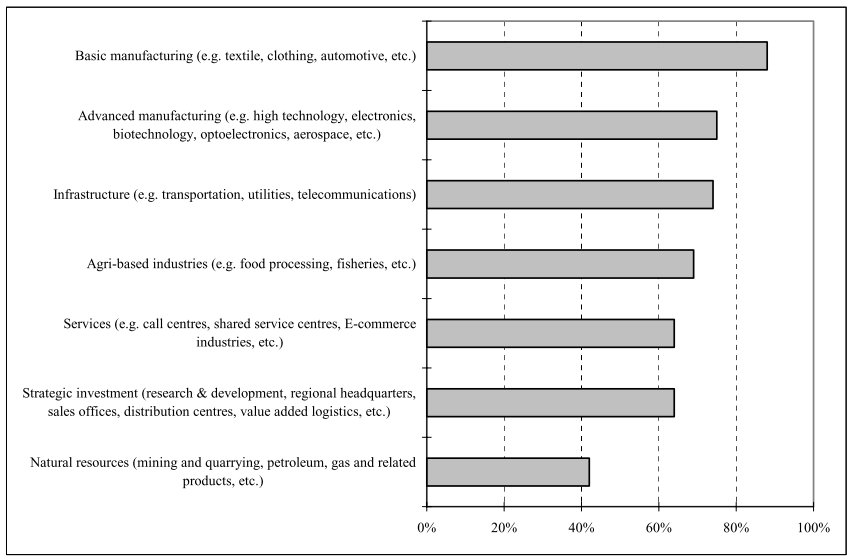
\includegraphics[width=\textwidth,keepaspectratio]{../figure/IPA_target_industries}
  \caption[Target industries by IPA around the world.]{Target industries by IPAs
    around the world. Because of the image building aspect of investment
    promotion, almost all IPAs say that they want to attract ``manufacturing,''
    ``advanced manufacturing,'' and ``infrastructure.'' Therefore, using what is
    listed as investment priorities may not be a reliable way to measure
    countries' preference for FDI. Source: \citet{UNCTAD2001}}
  \label{fig:IPA_target_industries}
\end{figure}

In sum, differentiating FDI by sectors only gives us a crude typology of FDI. We
can address this challenge using firm-level data, giving us information on not
only a firm's sector but also its operational characteristics, such as research
and development (R\&D) expenditure or export intensity. These measures are
firm-specific and get closer to what countries are looking for in FDI projects.
Using R\&D expenditure or export intensity as firms' characteristics in the
two-sided matching model, I will be able to estimate countries' preferences for
these traits.

\subsection{Measuring MNCs' activities}

As \citet{Kerner2014} argues, the IPE literature on FDI is a bit of a misnomer.
Political scientists are rarely interested in FDI \textit{per se}---rather, they
are interested in the activities of MNCs, which in turn, affect other important
issues such as nation-state autonomy \citep{Mosley2005}, economic development
\citep{Moran1998}, labor standards \citep{Mosley2007}, and environmental
policies \citep{Prakash2007}. However, while the theory involves MNCs as the
central actor in the causal mechanism, the empirics often uses FDI flow as the
variable of interest. These two concepts---the level of MNCs' affiliate
activities in a country and FDI inflow into a country---are not the same.

Consider the definition of FDI from UNCTAD, the main producer of FDI data widely
used by researchers:

\begin{quote} FDI has three components: equity capital, reinvested earnings and
  intra-company loans.
  \begin{itemize}
  \item Equity capital, i.e. the foreign investor’s purchase of shares of an
    enterprise [in the host country].
  \item Reinvested earnings, i.e. the foreign investor’s share \ldots of
    earnings not distributed as dividends by affiliates, or earnings not
    remitted to the foreign investor.
  \item Intra-company loans between direct investors and affiliate enterprises.
  \end{itemize} \citep[245]{UNCTAD2007}
\end{quote}

In essence, FDI data captures the amount of capital that crosses border. It is a
poor proxy for the scale of MNCs' activities in the host country because it
overlooks important components of MNCs' activities while including components
that are only relevant for balance of payment statistics
\citep{Beugelsdijk2010}.

Consider the argument that FDI is the driver for the diffusion of labor
standards across countries. \citet{Mosley2007} theorizes that FDI can have this
effect through three channels. First, MNCs may pressure the host government for
better rule of law and social programs. For MNCs to be able to effectively exert
this pressure, they must prove themselves valuable to the government by
providing jobs or tax revenue. Both of these factors are tenuously related to
the amount of foreign capital inside the host country. Indeed, an MNC can employ
thousands of employees, pay millions in tax, but show up as a net 0 on FDI flow
data because the profit is repatriated to the foreign investor or through
intra-company loans.\footnote{The issue of intra-company loans is particularly
  fraught with issues because companies very frequently use intra-company loans
  to get out of paying tax in a country. These loans will be recorded on the
  book as a massive outflow, even though the MNC still has a large presence on
  the ground.} The scale of MNCs' operation is further understated because FDI
statistics does not take into account capital raised locally. Also not included
is the superior productivity of MNCs, which acts as an important multiplier when
translating the amount of capital to the amount of output.

Second, scholars argue that MNCs may bring along best practices for workers'
rights and spread it to local firms. If this spillover effect happens via
competition, i.e. MNCs providing better working condition and forcing local
firms to compete, then MNCs must employ a lot of labor for this effect to be
noticeable. Or if the spillover happens via demonstration, then MNCs must form a
lot of linkages with local firms, as suppliers and buyers, for the diffusion of
norms to happen. Both the size of the labor force and the type of linkages with
the local economy are not captured by FDI flow statistics.

Third, scholars argue that MNCs may care more about labor quality than its cost,
and thus may invest in higher wages, better benefits, or more training. Once
again, for this effect to be noticeable, the MNC's industry, size of labor
force, and investment in productivity all matter a lot more than how much
capital it brings in and out of the country. In addition, non-equity
transactions between the parent company and the subsidiary, such as transfer of
knowledge, technology, and management practices, are not counted in FDI flow
statistics, thus excluding another component that is arguably much more
important to labor quality than the amount of capital.\footnote{These issues are
  not isolated to studies of FDI and labor standards, but are common to the
  whole IPE literature of the effect of FDI on policy convergence, such as
  environmental policies \citep{Prakash2007}.}

This mismatch between theory and empirics may also be a reason behind the
unsettled debate on the effect of FDI on poverty reduction. Scholars have
theorized that FDI can lead to economic development through three channels:
cheaper goods, technology transfer, and tax revenue. Once again, the causal
variable in the second and third channels is the scale and the type of MNCs'
activities in the host country, not necessarily the amount of capital crossing
the border. Indeed, productivity spillover is highly conditional on the
technological capability of the MNC and whether it forms thick linkages with the
local suppliers. The effect of FDI via tax revenue is also fraught with issues,
as MNCs frequently use intra-company transactions to artificially reduce book
profit and get out of paying tax \citep{Malesky2015c}.\footnote{These tactics
  are called ``transfer pricing,'' and can include tactics such as charging for
  internal intellectual properties and services whose price can be set
  arbitrarily by the firm} Since FDI flow statistics do not record these
intra-company transactions, it is not surprising that researchers reach the
confusing conclusion that FDI does not generate tax revenue.

What about studies that use FDI as the dependent variable, and are thus perhaps
interested in the flow of capital in and of itself?\footnote{Arguably, political
  scientists are not interested in the flow of capital in and of itself, but
  because of its implications for development, state autonomy, and other effects
  on policy. The discussion above has shown how problematic it is to study these
  effect of FDI using FDI flow data.} The vast majority of these studies on the
determinants of FDI flow rely on the ``obsolescing bargain'' model. Originally
developed by \citet{Vernon1971}, the model is so named because the bargaining
dynamics between the MNC and the host government changes over time, initially
favoring the MNC and gradually tips towards the host government as the MNC
commits more fixed capital on the ground. Indeed, knowing that it is costly for
the MNC to uproot its increasingly large and immobile operation, the host
government can unilaterally alter the original bargain, most egregiously by
expropriating the MNC's asset and profit, but more often via ``creeping
expropriation,'' e.g. increased tax or tougher regulation \citep{Li2009a}.
Political economists argue that MNCs are acutely aware of the ``obsolescing
bargain,'' and thus prefer to invest in countries whose governments can make a
credible commitment that they will not alter the original deal. This argument
translates into a large literature claiming that MNCs prefer countries with
democratic accountability \citep{Jensen2003}, a federal system
\citep{Jensen2005}, membership in international trade agreements
\citep{Buthe2008}, less political risk \citep{Beazer2011, Graham2010}, or more
veto points \citep{Choi2008}.

The linchpin of this argument is the assumption that FDI capital is illiquid and
cannot be quickly removed from the host country at will. This assumption is not
fully warranted. According to the US Bureau of Economic Analysis (BEA)'s 2004
survey, 43\% of US MNCs' balance sheet comprises of liquid assets that can be
liquidated within one year under normal operating situations. Among the 57\% of
the balance sheet that are illiquid, 24\% are ``other non-current assets,''
which include non-tangible assets like brand names, trademarks, and
patents---some of which are not expected to be liquidated but can be easily
removed from host countries. Only another 24\% of the balance sheet is made up
of physical capital, i.e. Plant, Property, and Equipment (PPE), which cannot be
easily moved and match most closely to what we have in mind as the ``illiquid
capital'' in the obsolescing bargain model \citep[113]{Kerner2014a}. Since FDI
flow data does not distinguish between liquid and illiquid capital, it is
suspect to use FDI flow data to test the ``obsolescing bargain'' argument,
calling into questions the entire literature on the political determinants of
FDI.

Besides the conceptual mismatch between FDI flow and MNCs' activities, from a
statistical standpoint, this measurement error may also be a contributing factor
to why there is little consensus in the FDI literature. Even if the measurement
error is random, it will inflate the standard error of our estimate when FDI is
the dependent variable, and bias our estimate towards 0 when FDI is the
independent variable. These effects may explain \citet{Jensen2012}'s surprising
finding that lower corporate tax rate does not lead to more FDI flow, or the
mixed empirical evidence for the relationship between FDI and development
\citep[108]{Mold2004}.

Even more worryingly, the measurement error is unlikely to be
random.\footnote{See \citet{Gallop2017} for a recent and more comprehensive
  discussion of measurement error in political science research.} For example,
the amount of locally raised capital---an important source of capital for MNCs
yet not captured in FDI flow data---is likely to correlate with how developed
the local capital market is or how wildly the exchange rate fluctuates.
Similarly, repatriated earnings, which does not necessarily indicate reduced
MNCs' activities but is recorded as an outflow in FDI flow data, is likely to
correlate with the tax rate of not only the host country but also other tax
havens that the MNC may have an affiliate in.

To deal with this measurement error problem, scholars have attempted to use
measurements that are closer to the theory than FDI flow. Given that political
scientists are often interested in MNCs' activities, recent work emphasizes
using MNCs' operational data directly. These firm-level datasets allow
researchers to measure directly the quantities of interest. For example,
re-visiting \citet{Li2009a}'s hypothesis that democracies are more attractive to
MNCs, \citet{Kerner2014} uses data on US MNCs' fixed capital expenditure to more
precisely test the relationship between democratic institutions and FDI
\textit{illiquid} capital, not just FDI in general. The author finds that there
is no relationship between democratic institutions and FDI flow, but there is a
positive relationship between democracy and MNCs' fixed capital expenditure,
confirming the theoretical expectation. Similarly, when \citet{Jensen2008a}
re-examines whether MNCs favor democratic regimes because they pose less
political risk, the author avoids using FDI flow and relies on price data of
political risk insurance agencies instead.\footnote{Scholars in other areas of
  IPE are also paying more attention to the issue of measurement error and the
  mismatch between empirics and theory, e.g. \citep{Karcher2013}.}


\section{Next steps}

In sum, the current FDI literature would benefit from focusing on countries'
preference for FDI, distinguishing types of FDI, and using firm-level
operational data instead of aggregate FDI flow statistics. While the theoretical
needs are clear and firm-level data has become more abundant in recent years,
political scientists have not developed a model to estimate this data structure
appropriately.\footnote{Examples of firm-level data include the US Bureau of
  Economic Analysis (BEA)'s survey of all US firms abroad, Tokyo Keizai's
  Overseas Japanese companies database (\textit{Kaigai Sinshutsu Kigyou
    Souran}), World Bank's Enterprise Survey, and Orbis database of companies
  worldwide.}

Very often, given the data structure of a set of firms interacting with a set of
countries, scholars resort to a dyadic-based analysis perhaps due to its being a
familiar tool. In such analysis, the unit of observation is a firm-country dyad,
and the model used is typically OLS regression. Each dyad is assumed to be
independent of each other, and any bias caused by interdependency is fixed via
post-estimation procedures, such as clustered standard errors \citep{Dorff2013}.
Unfortunately, this dyadic approach is patently inappropriate to analyze MNCs'
investment location. Indeed, once a firm chooses to invest in a country, it is
by definition not investing in another. Therefore, the values of firm-country
dyads deterministically constrain one another and cannot be modeled as
independent draws from a common distribution.\footnote{As a recent example,
  \citet{Arel-Bundock2017} uses Orbis, a global dataset of firms, to study the
  location decision of MNCs. The author uses random forest, a non-parametric
  machine learning approach, to predict whether an investment materializes for
  each of MNC-country dyad. However, because the predictors in the random forest
  model are dyad-specific, this approach cannot model interactions between
  dyads. In addition, since random forest does not produce interpretable
  coefficients, this black-box approach does not allow us to understand the
  preference of actors, how these preference are correlated with other
  characteristics, and how they may evolve over time.}

I propose using the two sided matching model to simultaneously address all of
these three issues in the literature. This approach models the matching process
explicitly, thus taking into account the dependency across dyads. The matching
process is made up of actors maximizing their utility functions---therefore, we
gain direct insight into what countries and MNCs value the most. Finally, the
model uses firm-level operational data, circumventing the measurement error
problem of aggregate FDI flow statistics. In the next chapter, I describe in
details how the two-sided matching model is set up and estimated.

%%% Local Variables:
%%% mode: latex
%%% TeX-master: "AnhLe_dissertation.tex"
%%% End:
}
\chapter{Two-Sided Matching Model}
\label{chap:model}

Here I present a behavioral model of the two-sided matching market, focusing on
the case of many-to-one matching, proposed by \cite{Logan1996}. For easier
exposition, throughout the chapter I will use the example of the labor market,
where many workers can be matched to one firm.

We assume that the matching process in the labor market happens in two stages.
In the first stage, each firm evaluates each worker in the sample, deciding
whether to hire that worker or not. At the end of this stage, each worker will
have received a set of offers from firms, which we call his \textit{opportunity
  set}. In the second stage, each worker evaluates the firms in his opportunity
set and chooses the firm that he likes best. This constitutes the final,
observed match between a worker and a firm. This is a many-to-one matching
problem because a firm can make offers to multiple workers, none, some, or all
of which can be accepted by workers.

Our model only needs data on 1) the covariates of firms and workers, and 2) the
job that workers accept. Such data is widely available in many social science
surveys of the job market. Importantly, we do not need to observe the opportunity
set. Therefore, our model obviates the need to follow the matching process and
record who makes offer to whom, which is rarely possible for researchers.

If we assume that firms and workers are utility-maximizing agents, at the end of
the matching process, no firm or worker would voluntarily change their final
matches. As discussed in Section~\ref{sec:game_theory}, this property is called
\textit{stability} in the game theoretic two-sided matching literature. We want
our model to have this property because matching markets tend to produce stable
matching. Indeed, \citet{Roth1992} show that for any given set of preferences, a
stable match always exist. Furthermore, \citet{Roth2016} and \citet{Adachi2003}
show that a decentralized market with agents making independent,
utility-maximizing decisions can also reach a stable match by itself.

This stability property does not imply that the matches will never change.
Indeed, if actors' preference shifts, their characteristics change, or new
actors enter the market, the matches will also change as a result of actors'
recalculating their utility and adjusting their decisions. Therefore, since we
are estimating actors' preference using only a snapshot of matching market, we
are making the assumption that on a systemic level, the average characteristics
of the actors and their preference remain sufficiently static for our estimates
to be meaningful.

This chapter will proceed as follows. First, I discuss the utility model for how
firms make offers to workers. Second, I discuss the utility model for how
workers choose the best offer among those extended by firms. Third, I show how
we can use a Bayesian MCMC
approach to estimate the model. Fourth, I analyze US labor data and demonstrate how to
interpret the model's result.

\section{Modeling firms' decision making}

A firm $j$'s decision on whether to hire worker $i$ rests on two utility
functions. First, firm $j$'s utility for hiring worker $i$ is:

\begin{align}
  U_j(i) &= \bm{\beta}_j' X_i + \epsilon_{1ij}
\end{align}

where $\beta_j$ is a vector of firm $j$'s preference for worker characteristics,
$x_i$ is a vector of worker $i$'s measured values on those characteristics, and
$\epsilon_{1ij}$ is the unobserved component that influences firm $j$'s utility.

On the other hand, the utility of not hiring worker $i$ is:

\begin{align}
  U_j(\neg i) &= b_j + \epsilon_{0ij}
\end{align}

where $b_j$ is the baseline utility of firm $j$, and $\epsilon_{0ij}$ is the
unobserved component that influences firm $j$'s utility.

Firm $j$ will make an offer to hire worker $i$ if $U_j(i) > U_j(\neg i)$.
Relevant worker characteristics (i.e. $X_i$) that a firm may consider are age,
education, or experience. The corresponding $\beta$'s represent the firm's
preference for these characteristics.

This model makes two important assumptions about firms' hiring process. First,
whether a firm decides to hire worker A depends on the characteristics of worker
A alone, and it will continue to hire worker A even if worker B is no longer
available. In other words, firms regard workers as substitutes rather than
complements.\footnote{In the terminology of \citet{Roth1992}, firms are assumed
  to have ``substitutable preference,'' or firms' preference is assumed to have
  the property of substitutability. As discussed in
  Section~\ref{sec:game_theory}, this assumption is necessary to prove the
  existence of stable matching in the case of many-to-one matching.} This
assumption is not universally true. A Hollywood producer may want to hire two
specific lead actors for their chemistry, and if one is unavailable, the other
also has to be replaced. However, for large firms where workers are closer to
swappable cogs than unique superstars, this assumption is reasonable.

Second, the model assumes that the utility of hiring a worker does not depend on
how many other workers accept the offer. In other words, the firm is large
enough to employ all the workers to whom it extends offer without feeling the
effect of diminishing marginal productivity of labor. This assumption is less
restrictive than it may seem. Indeed, we can model the fact that the workers
under consideration are less productive than the previous batch of workers by
allowing firm $j$ to have a high baseline utility $b_j$. Therefore, we are not
assuming that there is never any diminishing marginal
productivity of labor, only that there is negligible diminishing effect between
the first and the last of the workers under consideration. This assumption is a
reasonable approximation if the firm's labor force is large compared to the
number of workers being considered.\footnote{While not concerned with
  diminishing marginal productivity, \citet{Roth1992} also assume that firms'
  quota, i.e. the number of workers they can accept, is sufficiently large to
  hire everyone in the set of workers under consideration. This assumption
  simplifies the proof that a stable match always exists in the case of
  many-to-one matching.}

In addition to the two above assumptions about the process of firm's decision
making, we make three parametric assumptions that are standard in the discrete
choice literature. First, we assume a linear utility function. Second, we assume
that the error terms $\epsilon_{1ij}, \epsilon_{0ij}$ are uncorrelated with one
another and across firms. Third, we assume that the as error terms
$\epsilon_{1ij}, \epsilon_{0ij}$ follow the Gumbel distribution.\footnote{The
  Gumbel distribution is very similar to the normal, only with a slightly fatter
  tail that allows for slightly more extreme variation in the unobserved
  utility. Its density function is $\exp^{-(x + \exp^{-x})}$, with mode 0, mean
  0.5772, and fixed variance $\frac{\pi^2}{6}$. In practice, the difference
  between using Gumbel and independent normal error terms is small
  \citep{Train2009}.} The choice of the Gumbel distribution is largely motivated
by convenience since it allows us to derive the probability of firm $j$ making
an offer to worker $i$ as the familiar binomial logit form:

\begin{align}
  Pr(o_{ij} = 1) &= Pr(U_j(i) > U_j(\neg i)) \\
                 &= Pr(\epsilon_{0ij} - \epsilon_{1ij} <  \bm{\beta}_j ' X_i - b_j) \\
                 &= \frac{\exp({\bm{\beta}_j'X_i})}{1 + \exp({\bm{\beta}_j'X_i})} \label{eq:prob_offer_ij}
\end{align}

The term $b_j$ is absorbed into $\bm{\beta}$ when we add an intercept term to
the covariate matrix $X$.

Once firms have made their offers, each worker $i$ will have a set of offers
from which to pick her favorite. We call this set of offers the
\textit{opportunity set} of worker $i$, denoted $O_i$. Since unemployment is
always an available option, every opportunity set includes unemployment as an
``offer.''\footnote{In our model setup, firms and workers decide sequentially,
  with firms making offers first in order for workers to have opportunity sets
  to choose from. While firms and workers in real life certainly do not act in
  this sequential manner, the idea of the opportunity set is still applicable.
  Workers in the real labor market may not know their exact set of offers, but
  they can certainly guess which firms are within their reach based on their
  characteristics and on guesses about firms' preference.}

The probability of worker $i$ obtaining the opportunity set $O_i$ is:

\begin{align}
  p(O_i | \bm{\beta}) &= \prod_{j \in O_i} p(o_{ij} = 1 | \bm{\beta}) \prod_{j \notin O_i} p(o_{ij} = 0 | \bm{\beta}) \\
                      &= \prod_{j \in O_i} \frac{\exp(\bm{\beta_j} ' X_i)}{1 + \exp(\bm{\beta_j}' X_i)}
                        \prod_{j \notin O_i} \frac{1}{1 + \exp(\bm{\beta_j}' X_i)} \label{eq:conditional_probability_of_offer}
\end{align}

\section{Modeling workers' decision making}

Worker $i$'s utility for the accepting an offer from firm $j$ is:

\begin{align}
  V_i(j) &= \alpha' W_{j} + v_{ij}
\end{align}

where $\alpha$ is a vector of workers' preference for relevant characteristics
of firms, $W_j$ is a vector of firm $j$'s measured values on those
characteristics, and $v_{ij}$ is the unobserved component that influences worker
$i$'s utility.

Worker $i$ evaluates all the firms in her opportunity set and selects the offer
that brings the highest utility. This decision of worker $i$ concludes the
matching process, resulting in the observed final match between a worker and her
chosen firm in our data.

We make two assumptions in modeling the worker's decision making. First, for
simplicity, we assume that all workers share the same set of preferences--hence
$\alpha$ does not have a subscript $i$. The model can be extended so that there
is heterogeneous preference among workers, either by estimating a separate model
for each worker type (i.e. no pooling) or by building a hierarchical model for
worker preference (i.e. partial pooling).

Second, we assume that the error term $v_{ij}$ are uncorrelated across $j$. In
other words, the unobserved factors in the utility of one job offer is
uncorrelated to the unobserved factors in the utility of another job
offer.\footnote{This assumption also gives rise to the Independence of the
  Irrelevant Alternatives (IIA) property. IIA implies that the relative odds of
  choosing between two alternatives depend only on the two alternatives under
  consideration. It does not depend on whether other alternatives are available
  or what their characteristics may be. Hence, other alternatives are considered
  ``irrelevant.''} This assumption is most likely not true: if worker $i$ values
some unobserved factors of an offer, she is likely to consider those same
factors in another offer as well. The hope is that we have modeled the observed
portion sufficiently well that the remaining unobserved factors are close to
white noise. In any case, this issue afflicts any application of discrete choice
models and is not unique to our setup.\footnote{The discrete choice literature
  has developed solutions for such correlated error structure, such as nested
  logit, probit, and mixed logit, that can be applied here if we suspect that
  the unobserved portion is strongly correlated.}

Similar to our model of firm's utility, our model of worker's utility has three
additional parametric assumptions that are standard in the literature. First, we
assume that utility is linear. Second, the error term $v_{ij}$ are uncorrelated
across $i$. Third, we model $v_{ij}$ having a Gumbel distribution so that the
probability that worker $i$ will accept the offer of firm $j$ out of all the
offers in its opportunity set $O_i$ takes the conditional logit form
\citep{Cameron2005}:

\begin{align}
  p(A_i = a_i | O_i, \alpha_i) = \frac{\exp(\alpha'W_{a_i})}{\sum\limits_{j:j \in O_i} \exp(\alpha'W_j)} \label{eq:conditional_probability_of_accept}
\end{align}

where $a_i$ is the index of the firm that $i$ accepts to to work for.
Unemployment is indexed as 0.

\section{Model estimation}

Our goal is to estimate the preference of firms and workers, i.e. $\beta_j$ and
$\alpha$. The key insight is that, conditional on the opportunity set being
observed, the model of firms' and workers' decision making is a straightforward
application of the binary logit and conditional logit model. Both models can be
estimated with familiar tools like Maximum Likelihood Estimation (MLE).

However, in most social science research problems, the researcher only observes
the final match $A$ and not the opportunity set $O$. For example, labor market
data typically does not include the set of offers a worker received (or would
have received if she had applied), while data on her current job is widely
available. Similarly in the marriage market or the FDI market, researchers often
do not have the data on the offers being made, and only observe the final
matching between men and women (i.e. who is married to whom) and between MNCs
and countries (i.e. which factory is located where).

\citet{Logan1998}'s solution to this problem is to use the
Expectation-Maximization (EM) algorithm, an iterative method capable of finding
the maximum likelihood estimates when the model depends on unobserved latent
variables (i.e. the unobserved opportunity set in this case)
\citep{Dempster1977}. Our innovation is to estimate the model using a Bayesian
MCMC approach, which offers several advantages. First, our MCMC approach
produces the full posterior distribution, making inference easy. In contrast, EM
only produces point estimates out of the box.\footnote{\citet{Jamshidian2000}
  propose a method for estimating the standard error of EM estimates. However,
  for hypothesis testing, we need further assumptions about the distribution of
  the EM estimates.} Second, our MCMC approach can be faster than EM when the
latent variable, i.e. the opportunity set, is high dimensional
\citep{Ryden2008}.\footnote{Indeed, our opportunity set $O$ is a $(I \times J)$
  matrix of 0s and 1s, where $I$ is the number of workers and $J$ is the number
  of firms. Thus, there are $2^{IJ}$ potential values for the opportunity set,
  which quickly becomes untenable even for a small number of $I$ and $J$. The
  high dimension of $O$ forces \citet{Logan1998} to reduce the data dimension by
  aggregating 17 employers in the data into 5 employer types, e.g. professional
  or blue collar jobs.} Third, within the Bayesian framework, we can naturally
put a hierarchical structure on firms' preference. This allows us to borrow
information across firms, producing more precise estimates even when there is
not a lot of data for a specific firm.

The rest of this section describes how we conduct model estimation.

\subsection{Estimating the model using Metropolis-Hastings}

We are interested in the posterior distribution of workers' and firms'
preference given the observed final match, i.e. $p(\alpha, \beta | A)$.
Unconditioned on the opportunity set, this posterior is difficult to derive or
sample from. Therefore, we instead sample from the augmented posterior
$p(\alpha, \beta, O | A)$, whose density is much simpler to derive.\footnote{See
  \citet{Tanner1987} for a discussion of such data augmentation techniques.}
Specifically,

\begin{align}
  p(\alpha, \beta, O | A) &= \frac{p(A | \alpha, \beta, O) p(\alpha, \beta, O)}{p(A)} \\
                          &\propto p(A|O, \alpha) p(O|\beta) p(\alpha) p(\beta) 
                            \label{eq:posterior_density}
\end{align}

where $p(A|O, \alpha)$ is derived in
\eqref{eq:conditional_probability_of_accept}, $p(O|\beta)$ is derived in
\eqref{eq:conditional_probability_of_offer}, $p(\alpha)$ and $p(\beta)$ are
prior distributions for $\alpha$ and $\beta$. A key insight of this equation is
that the acceptance of offers, i.e. $p(A|O, \alpha)$, depends only on the
opportunity set and on the workers' preference. Similarly, the opportunity sets,
i.e. $p(O|\beta)$, depend only on firms' preference.

Because the opportunity set $O$ is a discrete matrix of 0's and 1's, there is
not any convenient conjugate model for \eqref{eq:posterior_density}, making
Gibbs sampling impossible. Therefore, we use Metropolis-Hastings instead, a
technique to sample from an arbitrary distribution $p(\theta)$ using the
following steps:

\begin{enumerate}
\item Start from an arbitrary value of $\theta$
\item Generate a proposal value $\theta^*$ from the proposal distribution
  $q(\theta^*|\theta)$
\item Calculate the acceptance ratio $MH_{\theta} =
  \frac{p(\theta^*)q(\theta|\theta*)}{p(\theta)q(\theta^*|\theta)}$
\item Accept the proposed value $\theta^*$ with probability $\max(1,
  MH_{\theta})$
\item Repeat step 2-4 until convergence
\end{enumerate}

In our case, we will use symmetric proposal distributions, i.e.
$p(\theta^*|\theta)$ = $p(\theta | \theta^*) \forall \theta, \theta^*$, so that
the MH acceptance ratio simplifies to $MH_{\theta} =
\frac{p(\theta^*)}{p(\theta)}$. In addition, because preference parameters tend
to be correlated, we use an adaptive proposal distribution so that our MCMC
samples have a faster convergence rate \citep{Haario1999,
  Haario2001}.\footnote{Description of the Adaptive Metropolis procedure?}

Below we describe how to sample from the posterior of each parameter in the
model using the Metropolis-Hastings (MH) algorithm. More detailed derivation of
the Metropolis acceptance ratio is included in Appendix~\ref{chap:MH_ratio}. We
ensure that our derivation and implementation of the acceptance ratio is correct
using the unit-testing approach suggested by
\citet{Grosse2014}.\footnote{Describe the unit-testing framework to ensure the
  correctness of MCMC code?}

\subsection{Posterior of the opportunity set $p(O|A, \alpha, \beta)$}

For each worker $i$, we propose a new value $O_i^*$ by flipping random cells in
the current value $O_i$ from 0 to 1 and 1 to 0. Substantively, this is
equivalent to perturbing the opportunity set by randomly making new offers or
withdrawing existing offers. Note that this proposal distribution is indeed
symmetric because proposing $O_i^*$ from $O_i$ and proposing $O_i$ from $O_i^*$
both involve flipping the same cells in the opportunity set. Hence,
$p(O_i^*|O_i) = p(O_i|O_i^*) =$ the probability of selecting these particular
cells out of the opportunity set.

The Metropolis acceptance ratio for the proposed opportunity set $O_i^*$ is

\begin{align}
  MH_O &= \frac{p(O_i^* | A_i, \alpha, \bm{\beta})}{p(O_i | A_i, \alpha, \bm{\beta})} \\
       &= \frac{\sum\limits_{j:j \in O_i} \exp(\alpha'W_j)}{\sum\limits_{j:j \in O_i} \exp(\alpha'W_j) \pm \exp(\alpha' W_{j^*})} \times \exp(\pm \bm{\beta}_{j^*}'X_i)
\end{align}

where $\pm$ evaluates to $+$ if $j^*$ is a new offer being added to the current
opportunity set, and evaluates to $-$ if $j^*$ is an existing offer being
withdrawn from the current opportunity set.

To understand the intuition behind this formula for $MH_O$, consider the
scenario in which we propose a new opportunity set for worker $i$ by adding an
offer from firm $j$. Since worker $i$ now has one more choice to choose from, it
becomes less likely that worker $i$'s accepted job is the best choice. This
makes the proposed opportunity set less consistent with the observed data than
the current opportunity set, and $MH_O$ should decrease accordingly. This is
reflected in the formula for $MH_O$ by the $\exp(\alpha'W_{j^*})$ term in the
denominator.

On the other hand, whether we should add the offer to the opportunity set also
depends on firm $j$'s preference for worker $i$. If hiring worker $i$ brings firm
$j$ net positive utility (i.e. $\bm{\beta}_{j^*}'X_i > 0$), we should add the
offer. This is reflected in the formula for $MH_O$ by the multiplier
$\exp(\bm{\beta}_{j*}'X_i)$, which is larger than 1 when $\bm{\beta}_{j^*}'X_i >
0$.

\subsection{Posterior of firms' preference $p(\alpha|A, O, \beta)$}

At the beginning of the MCMC chain, we propose a new $\alpha^*$ using a Normal
proposal distribution centered on the current value $\alpha$ with a hand-tuned
diagonal covariance matrix. Later in the MCMC chain, the covariance matrix of
the proposal distribution is adapted based on past samples to take into account
the correlations across preference parameters \citep{Haario2001}.

The Metropolis acceptance ratio for the proposed $\alpha^*$ is\footnote{We
  log-transform the Metropolis acceptance ratio for better numerics.}

\begin{align}
  MH_\alpha &= \frac{\alpha^*|A, O, \beta)}{p(\alpha | A, O, \beta)} \\
  \log MH_\alpha &= \sum_i \Bigl[ (\alpha^* - \alpha)' W_{a_i} + \nonumber \\
                 & \log\left(\sum\limits_{j:j \in O_i} \exp(\alpha' W_j)\right) -
                   \log\left(\sum\limits_{j:j \in O_i} \exp(\alpha^{*\prime} W_j)\right) \Bigr] + \nonumber\\
                 & \log p(\alpha^*) - \log p(\alpha)
\end{align}

\subsection{Posterior of workers' preference $p(\beta|A, O, \alpha)$}

We propose a new $\bm{\beta}^*$ using a Normal, adaptive proposal distribution
similar to $\alpha$. Because $\bm{\beta}$ is high dimensional, with one set of
$\beta$ for each employer, in each MCMC iteration we randomly choose and update
only a part of $\bm{\beta}$.

The Metropolis acceptance ratio for the proposed $\beta$ is

\begin{align}
  MH_\beta &= \frac{p(\beta* | A, O, \alpha)}{p(\beta | A, O, \alpha)} \\
  \log MH_\beta &= \sum_i \left[ \sum_{j \in O_i} \left(\beta_j^{*\prime}X_i - \beta_j^{\prime}X_i \right) + \sum_{j} \left( \log(1 + {\exp({\beta_j^{\prime}X_i})) - \log(1 +  \exp(\beta_j^{*\prime}X_i})) \right) \right] \nonumber \\
                & + \log p(\bm{\beta}^*) - \log p(\bm{\beta})
\end{align}


\subsection{Posterior of $\beta$'s hyperparameters $\mu_{\beta}, \tau_{\beta}$}

As discussed above, the Bayesian approach to estimating our two-sided model
allows us to put a hierarchical structure on the preference parameter. Here, we
model firms' preference $\bm{\beta}$ as being drawn from the multivariate normal
distribution $MVN(\mu_{\beta}, \tau_{\beta})$, where $\mu_{\beta}$ is the mean
and $\tau_{\beta}$ is the precision.

When the prior $p(\beta)$ is also normal, we have a conjugate multivariate
normal model, where $\mu_{\beta}$ and $\tau_{\beta}$ are the parameters while
$\beta$ is considered the ``data''.

Since the model is conjugate, we can sample from the posterior of $\mu_{\beta}$
and $\tau_{\beta}$ with Gibbs sampling. Their full conditional distribution of
$\mu_{\beta}$ is:

\begin{align}
  p(\mu_{\beta}) &\sim MVN(\mu_0, \Sigma_0) \\
  p(\mu_{\beta} | \beta, \tau_{\beta}) &\sim MVN(m, V) \text{ where } \\
  V &= (\Sigma_0^{-1} + n \tau_{\beta})^{-1} \\
  m &= (\Sigma_0^{-1} + n \tau_{\beta})^{-1} (\Sigma_0^{-1}\mu_0 + n \tau_{\beta} \bar \beta)
\end{align}

The full conditional distribution of $\tau_{\beta}$ is:

\begin{align}
  p(\tau_{\beta}) &\sim \text{Wishart}(\nu_0, S_0^{-1}) \\
  p(\tau_{\beta} | \beta, \mu_{\beta}) &\sim \text{Wishart}(\nu, S^{-1}) \text{ where } \\
  \nu &= \nu_0 + n \\
  S^{-1} &= \left(S_0 + \sum (\beta - \mu_{\beta})(\beta - \mu_{\beta})^{\prime}\right)^{-1}
\end{align}

\section{Results for US labor data}

To be written ...
} % A regular chapter, starts with '\chapter{Title}'
\chapter{Simulation results}
\label{chap:simulation}

In this chapter, I simulate the matching process of a labor market, using real
data on
workers' and firms' characteristics and assigned model parameters. I then apply
the two-sided logit model to show that the model is able to recover the
underlying parameters and to diagnose the properties of the MCMC sampling. I
compare the results of the two-sided logit model with the one-sided conditional
logit model, showing that the one-sided approach produces biased estimates of
workers' and firms' preference. This result demonstrates how the one-sided
approach, despite being the default method for analyzing two-sided markets, can
be misleading and unable to disentangle the effect of one side's preference from
the other side's.

\section{Labor market data}

To ensure that my simulation result generalizes to real situations, I use real
data on workers' and firms' characteristics from the US General Social Survey
(GSS), 1982-1990.\footnote{I thank Professor Michael Newton and Professor John
  Allen Logan for sharing the dataset.} On one side of the matching market is 2149 workers, a representative sample
of US male workers between 25 and 44 years old.
Table~\ref{tab:labor_occ5_summary_employee} shows the summary statistics for
workers. On average, a worker is 33 ($\pm$ 5.7)
years old and has 13 years ($\pm$ 3.1) of education. 11\% of workers in our sample are
non-white.

\begin{table}[!ht]
  \centering
  \caption{Summary statistics of workers' education, age, and race. The data
    come from the GSS, 1982-1990, for male workers in the US between 25 and 44
    years old.}
  \label{tab:labor_occ5_summary_employee}

% Table created by stargazer v.5.2 by Marek Hlavac, Harvard University. E-mail: hlavac at fas.harvard.edu
% Date and time: Mon, Apr 02, 2018 - 13:50:38
\begin{tabular}{@{\extracolsep{5pt}}lccccc} 
\\[-1.8ex]\hline 
\hline \\[-1.8ex] 
Statistic & \multicolumn{1}{c}{N} & \multicolumn{1}{c}{Mean} & \multicolumn{1}{c}{St. Dev.} & \multicolumn{1}{c}{Min} & \multicolumn{1}{c}{Max} \\ 
\hline \\[-1.8ex] 
Years of education & 2,149 & 13.103 & 3.111 & 2 & 20 \\ 
Age & 2,149 & 33.524 & 5.716 & 25 & 44 \\ 
Non-white & 2,149 & 0.113 & 0.316 & 0 & 1 \\ 
\hline \\[-1.8ex] 
\end{tabular} 

\end{table}

On the other side of the matching market are five firms, representing five job categories:
professional, managerial, sales / clerical / services, manufacturing blue
collar, and other blue collar. Table~\ref{tab:labor_occ5_summary_employer} shows
their characteristics. \textit{Prestige} is the Hodge-Seigel-Rossi score, used
in the GSS to measure the prestige of a job \citep{Hodge1964,
  NORC2014}. \textit{Autonomy} is calculated as the odds of having a supervisor, multiplied
by -1 so that a higher score is associated with a higher level of
autonomy.\footnote{In other words, $\text{autonomy} = -\frac{P(\text{having a
      supervisor})}{P(\text{not having a supervisor})}$} The prestige and the
autonomy scores of a firm in our dataset is the average scores reported by
workers who currently work in that job categories. Unemployment by itself does
not have a prestige and autonomy score. Following \citet{Logan1996}'s study on
the labor matching market, I calculate them as 50\%
of the prestige of the last job held and as the average autonomy scores of all
workers \citep{Logan1996}.\footnote{Our measurement of firms' prestige may be
  biased if workers that have a high regard for a certain type of job tend to
  work in that kind of job. Here we are making the assumption that workers are
  largely homogeneous so that workers in different jobs still have the same
  opinion regarding a job's prestige. While it is a strong assumption, it is not
an extra burden since we have already assumed that workers have the same set
of preferences in the modeling step. In addition, in other applications, such
as the FDI market where MNCs are matched with countries, we can obtain objective
data on countries' GDP, growth, and human capital, etc.}

\begin{table}[!ht]
  \centering
  \caption{Firms' characteristics}
  \label{tab:labor_occ5_summary_employer}

% Table created by stargazer v.5.2 by Marek Hlavac, Harvard University. E-mail: hlavac at fas.harvard.edu
% Date and time: Mon, Apr 02, 2018 - 13:50:38
\begin{tabular}{@{\extracolsep{5pt}} lccc} 
\\[-1.8ex]\hline 
\hline \\[-1.8ex] 
Firm category & Prestige & Pr(Supervisor) & Autonomy \\ 
\hline \\[-1.8ex] 
Unemployment & $18$ & $0.204$ & $$-$0.256$ \\ 
Professional & $59.670$ & $0.163$ & $$-$0.483$ \\ 
Managerial & $48.141$ & $0.442$ & $$-$3.237$ \\ 
Sales, Clerical, Services & $34.545$ & $0.100$ & $$-$0.112$ \\ 
Manufacturing Blue Collar & $34.330$ & $0.071$ & $$-$0.077$ \\ 
Other Blue Collar & $34.035$ & $0.175$ & $$-$0.214$ \\ 
\hline \\[-1.8ex] 
\end{tabular} 

\end{table}

\section{Simulated matching process}

I assign values to workers' and firms' preference parameters, choosing values to
achieve some level of realism and to have a sample of workers in each job.
Table~\ref{tab:sim_labor_nojobs_utility_functions} describes the utility
functions. I normalize firms' utility of not hiring to 0 so that firm $j$ will
extend and offer to worker $i$ if the utility of hiring is positive (i.e.
$U_{j}(i) > 0$. The magnitude of the intercept can thus be interpreted as how
selective a firm is in making an offer. For example, professional and managerial
firms are highly selective with intercepts of $-24$ and $-22$, while the other
firms are less so with intercepts of $-9, -8$ and $-6$. The coefficients
represent how much a firm values a worker's trait. For example, managerial and
professional firms have a similar preference for a worker's education, with
coefficients of 1 and 1.3. On the other hand, managerial firm values a worker's age twice
as much as professional firm does, with coefficients of 0.2 and 0.1.

While the two-sided logit model can be extended to accommodate different worker types as well, for
this simulation I assume that workers have homogeneous preference, sharing one
utility function.

Each utility function has a random component, represented by the
Gumbel-distributed error term $\epsilon$. While normally distributed error is
more common in simulations, justified by the claim that the error term is
the sum of many independent unobserved variables, here I use the Gumbel
distribution so that the coefficient estimates from the two-sided logit model can be
directly compared with the true preference parameter values.\footnote{If I use
  normally distributed error terms, the coefficient estimates have to be divided
by $\frac{\pi^2}{3}$ to be comparable with the true values.} Practically the
Gumbel distribution is very similar to the normal distribution, and I discussed
the implication of using the Gumbel distribution in further depth in Section~\ref{sec:model_firm_decision_making}.

\begin{table}[!ht]
\centering
\caption[Utility functions used in labor market simulations.]{Utility functions
  of firms and workers used in labor market simulation. $x_{i1}, x_{i2}, x_{i3}$ are worker \textit{i}'s education, age, and race (nonwhite is coded as 1). $w_{j1}, w_{j2}$ are firm \textit{j}'s prestige and autonomy, with $j \in \{1, \dots, 5\}$. The $\epsilon$'s are Gumbel-distributed error terms.}
\label{tab:sim_labor_nojobs_utility_functions}
\begin{tabular}{lll}
\\[-1.8ex]\hline 
\textbf{Firms' utility functions}  &                                                                                     \\
Professional                         & $U_{j}(i) = -24 + 1.3 x_{i1} + 0.1 x_{i2} + 1 x_{i3} + \epsilon$         \\
Managerial                           & $U_{j}(i) = -22 + 1 x_{i1} + 0.2 x_{i2} + 1 x_{i3} + \epsilon$     \\
Sales, Clerical, Services            & $U_{j}(i) = -9 + 0.75 x_{i1} + -0.05 x_{i2} + 0 x_{i3} + \epsilon$ \\
Manufacturing blue collar            & $U_{j}(i) = -8 + 0.5 x_{i1} + 0.02 x_{i2} + 0 x_{i3} + \epsilon$   \\
Other blue collar                    & $U_{j}(i) = -6 + 0.5 x_{i1} - 0.01 x_{i2} + 1 x_{i3} + \epsilon$   \\
  \hline
\textbf{Workers' utility function} & $V_{i}(j) = 0.01 w_{j1} + 0.1 w_{j2} + \epsilon$                   \\
  \hline
\end{tabular}
\end{table}

With these utility functions, I simulate the matching process as follows:

\begin{itemize}
\item{First stage:} Each firm $j$ evaluates each worker $i$, calculating the utility of
  hiring. If the utility of hiring is positive, it will extend an offer.
  Unemployment is always an option for workers, and is thought of as a ``firm''
  that extends an offer to every worker. After
  this stage, we generate an opportunity set that is a $2149 \times 6$ matrix,
  in which cell $(i, j)$ is 1 if worker $i$ receives an offer from firm $j$ and
  0 if not. We typically do not observe this opportunity set matrix in real datasets.
\item{Second stage:} Worker $i$ evaluates each firm that extends him an offer in
  the first stage, calculating the utility of working for that firm. Worker $i$
  then chooses a firm (or unemployment) if it offers the highest utility. After this
  stage, we generate a choice vector that is a $2149 \times 1$ vector, in which
  cell $i$ equals $j$ if worker $i$ decides to work at firm $j$. This choice
  vector is what we observe in real datasets such as the GSS. 
\end{itemize}

\section{Simulation results}

I estimate the two-sided logit model using the MCMC approach described in
Chapter~\ref{chap:model}. I use $N(0, \text{sd}=10)$ as a weak and proper prior for the preference
parameters. The results below are from a MCMC chain of 50,000
iterations with a thinning interval of 5, resulting in 10,000 saved iterations.
To propose new samples in the Metropolis-Hastings algorithm, I use normal
distributions with a scale hand-picked by examining the trace plots of discarded runs.

Figure~\ref{fig:sim_labor_nojobs_alpha} shows the trace plots of the MCMC
samples for workers' preference. We see that the MCMC chain mixes well and
quickly converge to the true value indicated by the red line. This result gives
us confidence that the MCMC algorithm is implemented correctly and can achieve
convergence within a reasonable time frame.

\begin{figure}[!ht]
  \centering
  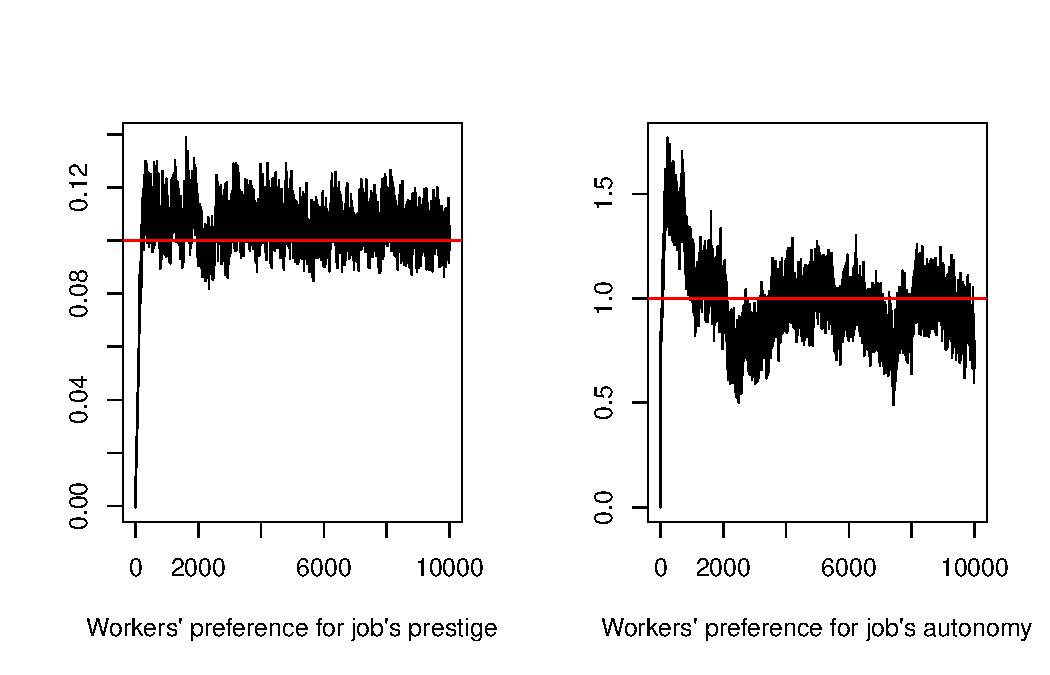
\includegraphics[width=\textwidth,keepaspectratio]{../figure/sim_labor_nojobs_alpha}
  \caption[Simulation result, estimate for workers' preference]{Two-sided logit estimates for workers' preference. The black line
    plots are the trace plots of the MCMC samplers, and the red line indicates the
    true parameter values. The trace plots show that the MCMC chain is able to
    converge to the true value after 10,000 iterations (2,000 saved iterations $\times 5$ thinning interval).}
  \label{fig:sim_labor_nojobs_alpha}
\end{figure}

Figure~\ref{fig:sim_labor_nojobs_beta_emp2} shows the trace plots of the MCMC
samples for professional firm's preference. We see that the MCMC chain is also
able to converge to the true parameter values, albeit slower and with more
autocorrelation between iterations.\footnote{To improve the mixing of the MCMC
  chain, I standardize workers' characteristics so that they have mean 0.
  Therefore, the intercept term has to be changed accordingly. The true
  intercept values displayed in the plots are the standardized intercepts, which
  is different from those reported in Table~\ref{tab:sim_labor_nojobs_utility_functions}.} There are several reasons for this poorer
mixing.

\begin{figure}[!ht]
  \centering
  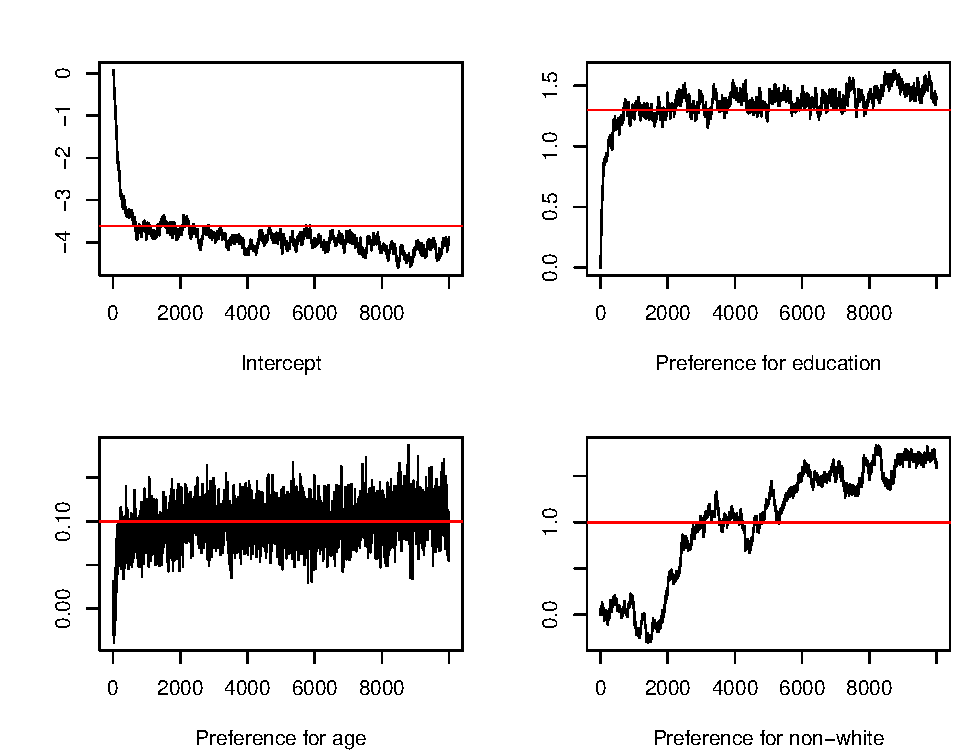
\includegraphics[width=\textwidth,keepaspectratio]{../figure/sim_labor_nojobs_beta_emp2}
  \caption[Simulation, estimates for professional firm's preference.]{Two-sided logit estimates for professional firm's preference. The
    MCMC chain is able to converge to the true parameter value, indicated by the
  red line, albeit with more autocorrelation than the MCMC chain for worker's
  preference in Figure~\ref{fig:sim_labor_nojobs_alpha}.}
  \label{fig:sim_labor_nojobs_beta_emp2}
\end{figure}

First, while we can use the entire sample to estimate the preference of
workers, only a subset of the sample works at a particular firm, resulting in a
smaller sample that we can use to estimate each firm's preference. This problem
is clearest in the trace plots for the managerial employer, which only has a
sample of 40 workers, or 1.9\% of the total sample \. To partially
combat this issue, I use a hierarchical model in which firms' preference
parameters are drawn from a common distribution. By doing so, I ``partially
pool'' the sample across firms, pulling the estimate for firms with small sample
sizes towards the common mean, and thus producing estimates that have more
predictive power \citep{Gelman2006}. On a related note, the MCMC chain of the
preference parameter for \textit{non-white} has a particularly poor mixing,
likely because \textit{non-white} is a binary variable, having less variation
and thus information that our model can use.

\begin{figure}[!ht]
  \centering
  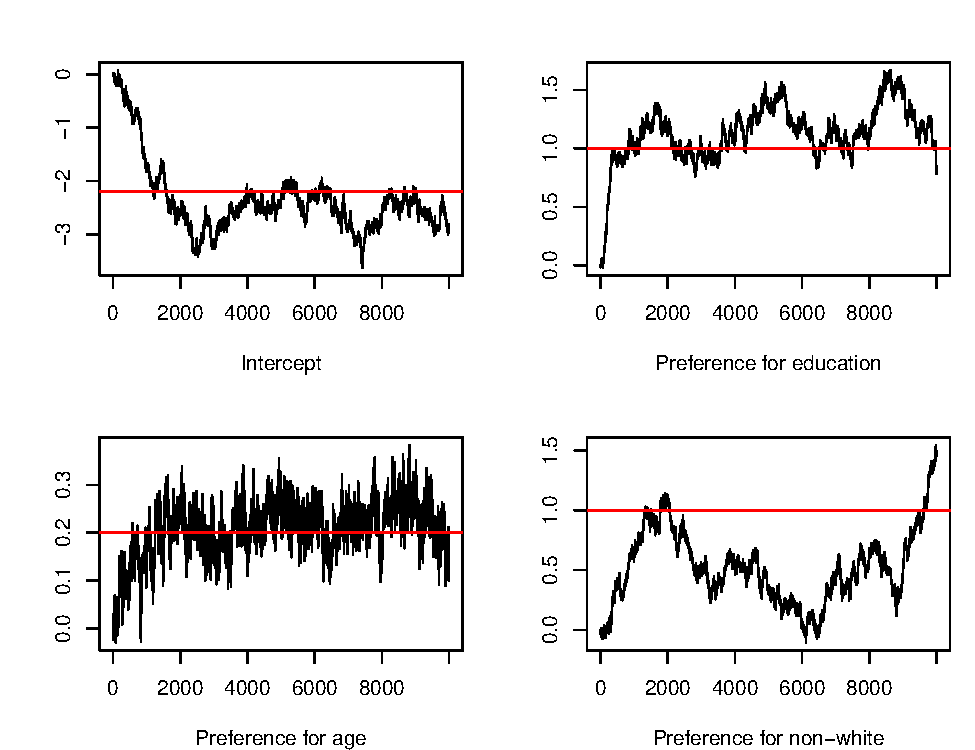
\includegraphics[width=\textwidth,keepaspectratio]{../figure/sim_labor_nojobs_beta_emp3}
  \caption[Simulation, poor mixing due to small sample size.]{Two-sided logit
    estimates for managerial firm's preference. Because the managerial firm only
  has a small sample size of 40 workers, or 1.9\% of the total sample, its
  preference is estimated more poorly than other's.}
  \label{fig:sim_labor_nojobs_beta_emp3}
\end{figure}

Second, while workers only have two preference parameters (for firm's prestige and autonomy), each firm has four
preference parameters (for worker's education, age, race, and an intercept
term), resulting in a total of 24 parameters. Updating the MCMC chain in such
high dimension is inherently difficult---to update one parameter we only need to
come up with one good proposal, but to update 24 parameters we need to come up
with good proposals for each of them.

Third, while firms' preference and the opportunity set are highly correlated,
our proposals for these parameters are independent, not take into their
correlation, and thus causing the MCMC to get stuck at local mode.
Section~\ref{sec:simulation_beta_opp_correlation} discusses this issue and
potential remedies in more details.

\section{Comparing two-sided logit model and one-sided models}

In this section, I demonstrate that, without taking into account the two-sided
nature of the matching market, one-sided models produce biased estimates of the
actors' preference. While it may be unsurprising that one-sided models fail when
the data generating process is so different from their assumptions, this is a
worthwhile exercise given that many empirical researches rely on these models.
For example, using discrete choice models (multinomial logit, conditional
logit), \citet{Cheng2006} models Japanese MNCs' location
choice across Chinese provinces, \citet{Aw2008} models Taiwanese firms' decision to
stay home or to open a factory in China and the US, and so do many others as
documented in \citet{Arauzo-Carod2010}.\footnote{In the empirical literature,
  researchers often use the term ``multinomial logit'' and ``conditional logit''
interchangeably to refer to a discrete choice model of unordered choices.
In this discussion, I follow the terminology in \citet{McFadden1994}'s seminal paper on discrete
choice models, distinguishing ``multinomial logit'' as the model whose
independent variables are the choosers' characteristics, and ``conditional
logit'' as the model whose independent variables are the choices' characteristics.} Using count models (Poisson, negative
binomial), \citet{Wu1999} models MNCs' location choice in Guangzhou, China, and
so do many others as documented in \citet{Guimaraes2003}. 

\begin{figure}[!ht]
  \centering
  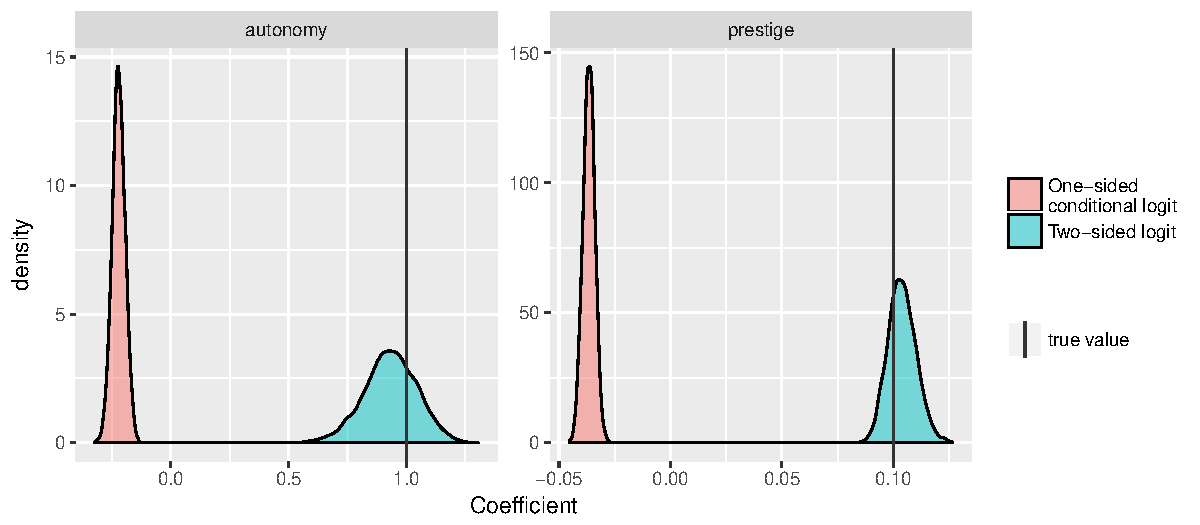
\includegraphics[width=\textwidth,keepaspectratio]{../figure/sim_labor_nojobs_alpha_tsl_vs_cl}
  \caption[Simulation, comparing the two-sided logit's and the
  one-sided conditional logit's estimate.]{Preference of workers, estimated by two-sided logit and conditional logit}
  \label{fig:sim_labor_nojobs_alpha_tsl_vs_col}
\end{figure}

\section{Interpreting two-sided logit result}

Discuss how to do interpretation

Simulate a change in one side leading to a wrong estimate of the other side
- Logan shows the change in the demand (i.e. the demand intercept)
- Maybe I could show the change in the preference for characteristics?
- This kind of simulation can be done again for FDI later

Discuss the effect of having offers that are different across respondents

\section{Issues with MCMC convergence}
\label{sec:simulation_beta_opp_correlation}
Discuss the correlation of MCMC

Discuss the adaptive procedure that I attempted but failed

The reason for the high degree of correlation is because beta and opp is highly
correlated
- We can't change the opp a lot, because conditional on beta, the opp is kinda
stuck. If we flip opp too much, it will be rejected because it'd be too
inconceivable given the current state of beta (may be make a graph here of the
rejection rate for opp)
- We can't change the beta a lot because conditional on opp, it's also kinda
stuck. This is especially true for countries with only a few observation of
firms invested in them.
Because if a country only has 5 firms in, if we flip the opp so that now the
country extends the offer to a new firm, and this firm is substantially
different from the current ones, that will really affect the estimate for beta.
For countries with a lot of firms invested in them, we can already estimate
their preference quite well, so flipping a new opp doesn't change the estimate
too much.
- Conceptually, we can think of a way to make proposal for beta and opp that
takes into account this correlation. For example, if we propose a new beta that
puts a high emphasis on employment, then we also are more likely to flip (to 1)
the cells that correspond to firms that have a large amount of employees.
However this is a bit too hard to implement and the computation cost may not be
worth it.

- The Gibbs sampler approach may work? But it's also unable to make correlated
move so may not be so much better.

blah

%%% Local Variables:
%%% mode: latex
%%% TeX-master: "../AnhLe_dissertation.tex"
%%% End:}
\chapter{FDI}
\label{chap:FDI}

\section{FDI trends}

Intro about studies of FDI in political science

Write about the economic literature on determinants of FDI

The political economy literature on the political determinants of FDI (and that
paper who shows that the political factors are not that important)

The studies on the preference of countries about FDI (Pandya, Pinto, and the
Harvard pub pol paper)


\section{Introduction}
\label{sec:introduction}

The political science literature on Foreign Direct Investment (FDI) has focused largely on how politics shapes the flow of FDI across countries. The central insight of this literature is that multinational corporations (MNCs) face an ``obsolescing bargain'' against the host government. Once the MNC has sunk its investment, it is vulnerable to the host government's changing regulations, backtracking on deals, or even expropriating its properties \citep{Li2009a, Sawant2010}. Certain institutional and political characteristics, such as numerous veto players, executive constraint, or strong property rights, allow the host government to make a credible commitment and thus ameliorate the severity of the ``obsolescing bargain'' problem \citep{Busse2007, Jensen2014, Li2003}. According to the literature, MNCs should invest more in countries with these characteristics.

This dominant approach in the literature has three long-standing issues that my paper will address. First, the majority of the literature relies on FDI stock and flow data as the outcome of interest even though they are often not an appropriate measure for the scale of MNCs' activities \citep{Kerner2014}. While it would be ideal to use firm-level data instead, both the lack of cross-national firm-level data and a suitable statistical model have posed a challenge.

Second, while there has been much focus on MNCs choosing host countries, the literature has largely neglected the other side of the investment decision: what are countries' preferences regarding MNCs? Consider the established finding that democracies receive more FDI. Without controlling for countries' preferences, it is difficult to interpret this fact as democracies actively pursuing MNCs or as MNCs finding democracies attractive. Not only are countries' preferences central to the modeling of investment decision, arguably it is also more steeped with politics and deserves more attention. \citet{Pinto2013} and \citet{Pandya2016} are two pioneering works in this area of research, proposing partisan politics and regime types as factors shaping countries' preferences for FDI. However, while their theories are ground-breaking, the empirical estimation of countries' preferences remains difficult.

Third, in addition to empirical issues raised above, I propose that we need to theorize about countries' preferences for FDI quality. While the political science literature has largely focused on the quantity of FDI, national policies and discourses pay much attention to the quality of FDI, using various incentives and restrictions to target certain types of FDI. Indeed, MNCs come with varying capital, demand for labor, and technology, all of which have different effects on the host country's economy. For example, policy makers and scholars have highlighted high-tech MNCs as a source of technological transfer for developing host countries, allowing them to upgrade their technical capacity and improve their productivity \citep{Findlay1978, Nunnenkamp2004}. While such high-quality FDI has been enthusiastically endorsed by the development community, I argue that only governments with a long time horizon want to attract high-tech FDI because technological transfer takes time to pay off.

In sum, the current literature would benefit from an analysis that is capable of using firm-level data to estimate both firms' and countries' preferences for each other's characteristics. To accomplish this goal, I adapt the two-sided matching model originally designed for the labor market and the marriage market. In this model, both firms and countries evaluate their available options and choose the best according to their utility functions. As in many social science contexts, we only observe the final firm-country matches and not the full set of available options (also known as the opportunity set). I solve this problem by using the Metropolis Hastings algorithm, a Markov chain Monte Carlo (MCMC) approach that repeatedly samples new opportunity sets and rejects them at an appropriate rate to approximate their true distribution. Since the two-sided matching model is derived explicitly from actors' utility functions, their parameters also enjoy a straightforward interpretation in the utility space instead of some aggregate outcomes.

The paper proceeds as follows. Section \ref{sec:literature_issues} discusses the
three long-standing issues with the literature and how they can be improved.
Section \ref{sec:model} lays out the utility structure in the two-sided matching
model and describes the matching process. Section \ref{sec:application} shows an
application of the model on a census of Japanese firms overseas. Section
presents the result. Section \ref{sec:conclusion} concludes.

\section{Three Issues in the Literature of FDI's Political Determinants}
\label{sec:literature_issues}

\subsection{Measuring MNCs' Activities}

For the majority of political science theory regarding FDI, the quantity of interest is the scale of MNCs' activities in a country, and not necessarily how much FDI crosses its border. Indeed, we theorize about how MNCs may reduce their activities for fear of expropriation, and how the host country's political factors can induce MNCs to invest more with a credible commitment not to expropriate. It is also the scale of MNCs' activities that determines how many jobs are created or how much of the domestic market is competed away, engendering labor's support and local business' lament.

However, to measure the scale of MNCs' activities, the vast majority of works uses how much FDI crosses the border, specifically FDI stock and flow \citep{Jensen2003, Ahlquist2006, Beazer2011, Graham2010}. As \citet{Kerner2014} points out, these measures, whose original purpose is to monitor balance of payments, are often misleading about MNCs' activities. FDI flow does not count locally raised capital and reinvested earnings since they do not cross any border. FDI stock calculated at market value fluctuates based on market price, unrelated to firms' behavior. FDI stock calculated at historical value, which records asset value at the time it was acquired, is more stable and appropriate to measure the scale of MNCs' activities. Unfortunately, due to onerous data requirements, most countries measures FDI stock by simply adding up FDI flow across years.

Given the interest of political science theory in MNCs' activities, \citet{Kerner2014} suggests less use of FDI stock and flow and more use of firm-level statistics. For example, consider the hypothesis that countries with more veto players have more stable policies and are thus more attractive to FDI \citep{Li2009a}. Instead of using FDI stock and flow into a country to measure its attractiveness, we can study whether more MNCs are located there.

While firm-level data has become more abundant in recent years,\footnote{Examples of firm-level data include the US Bureau of Economic Analysis (BEA)'s survey of all US firms abroad, Tokyo Keizai's Overseas Japanese companies database (\textit{Kaigai Sinshutsu Kigyou Souran}), World Bank's Enterprise Survey, and Orbis database of companies worldwide.} it is not clear how to analyze this type of data appropriately. Given the data structure of a set of firms interacting with a set of countries, one may consider a dyadic-based analysis, frequently used in the International Relations literature. In such analysis, the unit of observation is a firm-country dyad, and the model used is typically OLS regression. Each dyad is assumed to be independent of each other, and any bias caused by interdependency is fixed via post-estimation procedures, such as clustered standard errors \citep{Dorff2013}. 

Unfortunately, this dyadic approach is inappropriate to analyze MNCs' investment location. Once a firm chooses to invest in a country, it is by definition not investing in another. Therefore, the values of firm-country dyads deterministically constrain one another and cannot be modeled as independent draws from a common distribution.

The two sided matching model solves this problem by considering one firm-country match as the unit of observation. The intuition is as follows. If we observe that a firm is welcome to invest in countries $j_1, j_2, \dots, j_n$ but ends up investing in country $j^*$, it must mean country $j^*$ offers the highest utility to firms. Continuing the previous example, if country $j^*$ has more veto players than average, we can infer that MNCs indeed prefer countries with more veto players.

\subsection{Estimating Countries' Demand for FDI}

Recognizing that our model of investment location has not taken into account countries' demand for FDI, \citet{Pinto2013} and \citet{Pandya2016} recently broke ground in this area. Similar to the rich IPE literature in trade and exchange rate, these studies argue that countries' demand for FDI varies according to FDI's distributive effect on their domestic constituencies \citep{Broz2001, Milner2005a}. In this theoretical framework, labor supports FDI because foreign firms bring capital that increases the demand for labor and raises productivity, both of which lead to higher wage. On the other hand, domestic firms oppose FDI because foreign firms compete for local labor, inputs, and markets. Both \citet{Pinto2013} and \citet{Pandya2016} formulate their theories as a variant of this labor-vs-business tension, which surfaces in the former work as left-vs-right governments, and in the latter as democratic-vs-authoritarian regimes.

While these pioneering works have enriched our understanding of the relationship between politics and FDI, their empirical approaches do not satisfactorily measure countries' demand for FDI, leaving their theoretical arguments untested.

Consider \citet{Pinto2013}'s approach, which controls for economic and institutional factors that affect FDI flow into a country. The author then claims that the country's openness towards FDI is what's left in the residual.\footnote{Specifically, the estimation of FDI openness involves two steps. First, the author runs a gravity model explaining bilateral FDI flows, estimating the intercept as the host country-year fixed effect. Second, this fixed effect is then regressed on several economic and endowment factors of that country-year (i.e. GDP, GDP per capita, average school years, arable land). The residual in the second stage is considered the country's ``FDI openness'' in that year.} For this approach to be valid, every economic, institutional, and endowment factors that affect FDI flow have to be controlled for, leaving only the country's demand in the error term. This claim is much stronger than the regular assumption of exogenous and normally distributed error, which is valid as long as the omitted factors are uncorrelated with the independent variable of interest. Framed substantively, since the residual is likely to contain more than just the country's demand for FDI, if we observe an abnormally high level of FDI, we do not know whether it is because the country welcomes FDI or because MNCs find something attractive in the country.\footnote{In addition, the data requirement of bilateral FDI flows, ideally disaggregated by sectors, is very demanding. Therefore, this approach is limited to OECD countries only \citep{Pinto2008}. During the period the authors study, 1980-2000, OECD countries accounted for 95\% of global FDI outflow and 90\% of inflow. However, since then the role of the developed world in global FDI has declined sharply, reduced to 60.8\% of outflow and 40.6\% of inflow in 2014 \citep{UNCTAD2015}.}

In contrast to \citet{Pinto2013}'s statistical approach, \citet{Pandya2014, Pandya2016} substantively measures countries' demand for FDI, using the annual US Investment Climate Reports to code the number of industries that have foreign ownership restrictions or face investment screening. The advantages of this measurement are its ease of interpretation and its availability for many countries. However, two problems remain. First, adding up the raw count of restricted industries is not appropriate because industries are not all the same. For example, given the reach of the banking sector into all corners of the economy, a country's opening up its financial industry indicates much more FDI-friendliness than, say, allowing foreign furniture makers to set up shops. Since the theoretical argument is driven by FDI's distributive effect, it is suspect to ignore the varying impact of FDI across sectoral constituencies. 

Second, according to the coding rules, an industry is coded as free if there is
no mention of restriction. If an industry receives little FDI, it may not be
worth mentioning as being restrictive and yet still coded as open. Therefore,
``zero restriction'' in the dataset can either mean that a country is very
closed or very open to FDI. This concern is not hypothetical. Figure \ref{fig:china_fdi_restriction} shows that, following the coding of the US Investment Climate Reports, China seemed 100\% open to FDI up until 1986 when it started imposing restrictions. The reality is the opposite. Prior to 1986, only limited FDI was allowed as joint-venture in Special Economic Zones (SEZ). The year of 1986 was, in fact, the first time China allowed any wholly owned FDI outside of SEZs.

\begin{figure}[!ht]
\centering
\includegraphics[width=0.75\textwidth,keepaspectratio]{../figure/china_fdi_restriction}
\caption{China's FDI Ownership Restriction, as coded in \citet{Pandya2010}. Prior to 1986, FDI in China was limited to few experimental Special Economic Zones, and thus not mentioned in US Investment Reports. The sharp spike in 1988 also does not seem to correspond to any actual change in policy, and likely another artifact of reporting. (See \citet{Zebregs2002} for a historical overview of China's FDI policy.)}
\label{fig:china_fdi_restriction}
\end{figure}

The two-sided matching model circumvents these thorny measurement issues by incorporating countries' utility function directly into the model. If we observe that country $j$ welcomes firms $i_1, i_2, \dots, i_n$ to invest but not others, we can compare the characteristics of firms $i_1, i_2, \dots i_n$ with the others to infer country $j$'s preference.


\subsection{Estimating Countries' Preferences for FDI's Technological Intensity}

While the political science literature has focused almost exclusively on the quantity of FDI, treating all FDI as one homogeneous flow of capital, policy makers seem to pay much more attention to distinguishing types of FDI. Commenting on the role of International Investment Agreements (IIAs), \citet{UNCTAD2015} says, ``Today, increasing the quantity of investment is not enough. What matters is its quality, i.e. the extent to which investment delivers concrete sustainable development benefits.'' Governments in developing countries, from Ghana to China, all offer various forms of tax incentives and fee waivers to attract FDI that invests in a remote region, brings new technology, or focuses on exporting \citep{Ricupero2000}. Since 2006, China's official FDI policy has been ``quality over quantity,'' promoting FDI with intense R\&D in high-productivity sectors \citep{Guangzhou2011}. Indeed, for developing countries, the hope is that MNCs will transfer their technologies to the domestic economy by training workers or partnering with local suppliers.

Despite the importance of disaggregating FDI by its quality, data unavailability remains the bottleneck. The few existing attempts use detailed data from only one country or limit the sample to OECD countries \citep{Alfaro2003, Alfaro2007, Javorcik2004}. With cross-country firm level data now available, we often have information on the firms' industry or even research and development (R\&D) expenditure. With the two-sided matching model, I will be able to estimate countries' preferences for firms' technological intensity. I hypothesize that, since MNCs' technologies takes time to diffuse to local businesses, a country' preference of high-tech FDI is shaped by its time horizon.

\section{Using firm level data in FDI studies in Political Science}

Look at Kerner2014

Look at studies in FDI across China

\section{The literature on Japanese MNCs investment}

Make a graph about the size of Japanese FDI relative to Asia FDI here

Calculate the size of Japanese FDI into several countries (nominator from JETRO,
denominator from IMF)

Relative exchange rate (Takagi2011). Assume that the capital market is
imperfect, that external borrowers face a premium. So if a host country currency
depreciates, inflow FDI will increase because the same amount of source currency
can buy more input in the host country. The relationship is especially strong
between exchange rate and inflow of FDI into industries with a lot of
firm-specific assets. (e.g. Japanese firms buy a US firm with innovation for
cheap, then use that innovation to improve its production back home in yen) 

(Originally people don't think exchange rate matter because if you can buy an
asset for cheap in the host country, when you repatriate the profit back to the
home country it's a wash)

FDI is all about the relative factors (because a firm thinks about a country in
terms of how that country is relative to its host). So the two sided matching
framework makes sense

General FDI: Why don't firms export or license, but open their own plant
overseas? Argument is that they have firm-specific asset that cannot be fully
exploited otherwise. A licensee won't be able to exploit the entire asset, both
sides can't agree on a price beforehand (This is the OLI framework,
ownership-location-internalization, also the internationalization hypothesis). Empirically, firm specific asset is
unobservable, so people use R\&D intensity and advertising intensity instead.
R\&D does correlate strongly with multinationality.


\section{Applying the Two-Sided Matching Model to Japanese MNCs}
\label{sec:application}

In this section, I apply the two-sided matching model to study the investment
location of Japanese firms overseas. The data comes from a dataset compiled by
Andrew Delios from \textit{Kaigai
  Shinshutsu Kigyou Souran} (Japanese Overseas Investments-by Country), between
1986-1999 editions, a publication that contains information
about the foreign affiliates of listed Japanese firms.\footnote{I thank Professor Andrew Delios for
  generously sharing the data.} Tokyo Keizai, Inc. collect these data via annual
surveys of the overseas operations of both listed and non-listed firms. This database is reputed to include all Japanese
firms overseas \citep{Yamawaki1991}. \citep{Delios2001} compares the coverage of
the Japanese Overseas Investment with other sources of publicly listed firms and
found that 98.5\% of public firms are included, which has 99.5\% of the foreign
subsidiaries. Since there is no public information on non-public firms, they
cannot check the coverage of the Japanese Overseas Investment for these firms.
However, the result for the public firms makes us confident that our data is
close to the population of Japanese FDI overseas.\footnote{There are similar
  datasets if scholars want to replicate this study in other context. On a
  global scale, the ORBIS dataset claims to have data of FDI firms across
  countries. (cite the paper that I reviewed). However, there are concerns about
  its data quality, given that the data is collected via public governmental or
  municipal sources. Due to the differences of reporting across jurisdiction,
  the data quality is much less consistent than the Japanese Overseas Survey. For the US, there is a census of
  US firms overseas, which should be similarly high quality. However, this
  dataset requires citizenship. Tokyo Keizai, Inc. also continue to publish this
data series. However, the cost is prohibitive and require understanding Japanese
to work with.}



Sample choices:

- I only use the data of subsidiaries that are founded in year 1996 (which is
different from the list of companies who are in existence in year 1996). Reasons:
+ the utility function is only modeled as a linear combinations of the country /
firms covariates. It does not take into account the cost of uprooting a firm to
move to another country once they are already there. This is important for FDI
because, unlike equity investor, FDI are less foot-loose. Indeed, the fact that
it is not footloose is an important quality of FDI that's appealing to countries
(cite). The political economy literature on FDI has also derived its insights
largely from this ``obsolescing bargain'' problem, so it's important that our
model takes this into account. In past applications of the two sided matching
approach, researchers use a random sample in time (i.e. a sample of all couples
who's married in a certain year), which is fine, because the
cost of leaving a job or leaving a partner may not be too onerous. However, for
FDI, this fixed cost is more central. By limiting the sample to the firms who
are founded in 1996, we examine their decisions as they are all looking for
potential locations.\footnote{Of course, a subsidiary's foundation year in 1996
  does not preclude the decision process to happen outside of this year.
  However, I consider this a reasonable approximation, given that many country
  characteristics, especially the political and institutional ones, do not
  change drastically within a window of several years.}

+ the data is largest for this year. (some summary statistics here). There may
be some concerns about this year being a special year, in the year leading up to
the 1997 Asian Financial Crisis. But 1) we're only looking at manufacturing
firms, not equity investors or land developers, 2) FDI during the crisis is
largely the same as before the crisis \citep{UNCTAD1998}. Indeed, this is
because FDI firms are largely looking at countries' fundamentals, such as labor
cost, market potential, and thus not affected by the fluctuations in the
financial markets. Essentially, the types of firms that invest before, during,
and after crisis are still the same types of firms.\footnote{One potential
  concern is that our data does not capture the firms who thought about making
  an investment but decided not to. This could be a problem if the MNCs in our
  dataset is the most risk-seeking firms, then essentially we've only estimated
  the preference of the very risk-seeking or the very risk-averse firms. AFC too
high short term interest, too high local currency that is fixed. However, the
exit rate of Japanese firms in Thailand, the epicenter of the financial crisis,
is the same, indicating that the types of firms who invest are not so affected
by the financial crisis. Looking at the exit is the reverse way of looking at
who would have invested but didn't. \citep{Delios2001}}

+ I only consider Japanese FDI into East Asian and Southeast Asian economies to
make sure that it's realistic to say that all these companies have the same
preference parameters. \citep{Pak2005} finds that Japanese FDI in the West seeks
to augment their global competitiveness, while Japanese FDI in the East focuses
on exploiting their core competencies. Japanese FDI in the West are ones with
oligopolistic power in their domestic market (so they are in a strong position
to compete) and require R\&D and marketing capabilities. They have different
level of equities. This suggests that the two types of firms are fundamentally
different.\footnote{Even though the difference in theory could be due to the
  preference of the countries. However, it doesn't make sense why the level of
  Japanese ownership is also different (because countries would not care about
  this).} 

The final sample includes 6474 Japanese
foreign affiliates in 2003, spreading across 37 countries, with China and the US
leading as the two top destinations for Japanese MNCs (Table \ref{tab:list_of_countries}).

For firms' characteristics that countries consider, I include:

\begin{itemize}
\item Capital size (in US\$): A main argument for the benefit of FDI is that it brings capital to the country, improving labor productivity. MNCs' capital is especially important for developing countries, which cannot muster much domestic capital from their poor population. The capital size of a firm is included in the Japanese Overseas Business dataset.

\item Labor size: Similarly, a reputed benefit of FDI is that it creates jobs, generating not just economic growth but also increasing the government's popularity among the populace. The total number of employees of a firm is included in the Japanese Overseas Business dataset.

\item Technology intensity: I proxy for a firm's technology intensity by the
  industry to which it belongs. \citet{OECD2009} categorizes ISIC industries
  into four levels of technology intensity---low, medium low, medium high, and
  high---according to the level of R\&D expenditure divided by sales. I convert
  the industry classification of firms in my data from SIC 3 to ISIC and
  categorize their technology intensity from 1 to 4, with 1 being low and 4
  being high. On several occasions, one industry in SIC 3 matches to multiple
  ISIC (rev 3) industries or none at all. In the former case, I take the average
  across matched ISIC industries. In the latter case, the data is missing and
  later removed from the analysis.\footnote{\cite{Bergstrand2007} discusses the
    difference between R\&D intensity and advertising intensity, and find that
    R\&D intensity is higher for manufacturing firms compared with consumer
    product firms. Plus R\&D intensity is much more important for firms'
    performance than advertising intensity.}\footnote{Definition of R\&D
    intensity: the amount spent on R\&D as a percentage of sale}

\item Export intensity (ratio of export to sale):
\end{itemize}

Summary statistics table for these covariates.


For countries' characteristics that firms consider, I include:

\begin{itemize}
\item Market size: MNCs are expected to prefer countries with a large market
  size, which present MNCs with many potential customers. Indeed, this has been
  often cited as the allure of China to MNCs \citep{Luo2010}, as well as
  confirmed in larger studies. This is also a major variable in the gravity
  model, which has become a standard model for analyzing FDI flows.
  \citet{Bergstrand2007} provides the theoretical framework for the use of
  gravity model. I follow the standards in the literature and include log GDP
  (constant 2005 US\$), taken from the Penn World Table.\footnote{An advantage
    of the Penn World Table is that it compiles data for Taiwan, an important
    destination that the World Bank Development Indicators does not include.}

\item Level of development: MNCs are expected to prefer countries with a high
  level of development. A developed economy has consumers with high purchasing
  power and better infrastructure. It can also measure capital abundance, in
  which case a higher GDP per capita imply less flow because the simple model of
  FDI frames FDI as the movement of capital from the capital rich countries to
  the capital poor countries. To measure development, I use log GDP per capita
  (constant 2005 US\$) from World Development Indicators.

\item GDP growth may be a proxy of potential returns, 

\item Labor quality: As one primary factor of production, labor matters greatly to firms' productivity and profit. To measure labor quality, I use the average years of schooling of adult, taken from the UNDP's Human Development Report.\footnote{Since Taiwan is not included in UNDP's and World Bank's data, I collected its statistics from the Taiwanese Statistical Website.}

\item Democracy: Democracy has been a mainstay in the political science literature on FDI. Scholars have argued that MNCs want to invest in democratic regimes for various reasons, including stable policy, credible commitment, and strong property rights \citep{Ahlquist2006, Li2003, Jensen2003}. On the other hand, recent works have also argued that democratic regimes want FDI more than autocratic regimes \citep{Pandya2016}. Thus, it is unclear whether the observed high level of FDI in democracies is due to the push or the pull factors. By controlling for countries' preference in the two-sided matching model, I can better estimate the effect of democracies on firms' utility. I measure democracy using the binary Demoracy \& Dictatorship, developed by \citet{Cheibub2009b}.
\end{itemize}


\section{Conclusion}
\label{sec:conclusion}

In this paper, I propose the two-sided matching model to estimate firms' and countries' preferences, solving three persistent issues in the literature of FDI's political determinants. The results indicate that, for Japanese MNCs, only a country's level of development matters and not its market size, labor quality, or regime type. This finding suggests that we should take a closer look at the relationship between democracies and MNCs. Since previous works in the literature have not controlled for countries' preferences, they may have mistaken democracies' love for FDI as FDI's fondness for democracies.

On the other hand, the model's estimation of countries' preference remains lacking. Since each country has its own set of parameters, the parameter space seems too large for the current implementation of the Metropolis-Hastings algorithm to fully explore. Several solutions are possible. First, we can collapse countries into categories of interest, e.g. regime types, (categorical) time horizon length. Second, we can build a hierarchical model, modeling countries' preferences as draws from a common distribution. Such model will allow us to pool information across countries and reduce the parameter space.}
%==============================================================================

%-----------------------------------------------------------------------------%
% APPENDICES -- OPTIONAL. These are just chapters enumerated by Appendix A,
%                Appendix B, Appendix C...
%-----------------------------------------------------------------------------%
\appendix
\chapter{Derivation of the Metropolis-Hastings Acceptance Ratio}
\label{chap:MH_ratio}

\subsection{Opportunity sets $O$}

Target distribution for a firm $i$ 

\begin{align}
p(O_i | A_i, \alpha, \bm{\beta}) &= \frac{p(O_i, A_i, \alpha, \bm{\beta})}{p(A_i, \alpha, \bm{\beta})}
\end{align}

\begin{align}
MH_O = \frac{p(O_i^* | A_i, \alpha, \bm{\beta})}{p(O_i | A_i, \alpha, \bm{\beta})} &= \frac{p(O_i^*, A_i, \alpha, \bm{\beta})}{p(A_i, \alpha, \bm{\beta})} \times \frac{p(A_i, \alpha, \bm{\beta})}{p(O_i, A_i, \alpha, \bm{\beta})} \\
&= \frac{p(O_i^*, A_i, \alpha, \bm{\beta})}{p(O_i, A_i, \alpha, \bm{\beta})} \\
&= \frac{p(A_i | O_i^*, \alpha)p(O_i^*|\bm{\beta})}{p(A_i | O_i, \alpha)p(O_i|\bm{\beta})} \label{eq:updateO_joint_dist_into_conditional_dist} \\
\end{align}

where the factorization of the likelihood in \eqref{eq:updateO_joint_dist_into_conditional_dist} is due to the fact that the acceptance of firm $i$ only depends on what is offered to it and what is its preference, $p(A_i | O_i^*, \alpha)$; what is offered to $i$ depends on the preferences of all countries, $p(O_i^* | \bm{\beta})$.

If we plug in \eqref{eq:conditional_probability_of_accept} and \eqref{eq:conditional_probability_of_offer}

\begin{align}
\frac{p(O_i^* | A_i, \alpha, \bm{\beta})}{p(O_i | A_i, \alpha, \bm{\beta})} &= \frac{\sum\limits_{j:j \in O_i} \exp(\alpha'W_j)}{\sum\limits_{j:j \in O_i} \exp(\alpha'W_j) + \exp(\alpha' W_{j^*})} \times \exp(\bm{\beta}_{j^*}'X_i)
\end{align}

where $j^*$ is the index of the newly sampled job. This is the case when the newly proposed job is not already offered, so it's added to the opportunity set.

When the newly proposed job is already offered, so it's removed from the opportunity set, we have

\begin{align}
\frac{p(O_i^* | A_i, \alpha, \bm{\beta})}{p(O_i | A_i, \alpha, \bm{\beta})} &= \frac{\sum\limits_{j:j \in O_i} \exp(\alpha'W_j)}{\sum\limits_{j:j \in O_i} \exp(\alpha'W_j) - \exp(\alpha' W_{j^*})} \times \exp(- \bm{\beta}_{j^*}'X_i)
\end{align}

\subsection{Workers' parameters, $\alpha$}

Target distribution:

\begin{align}
p(\alpha | A, O, \bm{\beta}) &= \frac{p(O, A, \alpha, \bm{\beta})}{p(A, O, \bm{\beta})}
\end{align}

Metropolis-Hasting acceptance ratio:

\begin{align}
MH_\alpha = \frac{p(\alpha^* | A, O, \bm{\beta})}{p(\alpha | A, O, \bm{\beta})} &= \frac{p(A_i | O_i, \alpha^*)p(O_i|\bm{\beta})}{p(A_i | O_i, \alpha)p(O_i|\bm{\beta})} \\
&= \frac{p(A_i | O_i, \alpha^*)}{p(A_i | O_i, \alpha)} \label{eq:updatealpha_MHratio_final}
\end{align}

where \eqref{eq:updatealpha_MHratio_final} is due to the flat prior (so $\frac{p(\alpha^*)}{p(\alpha)}=1$) and the symmetric proposal distribution (so $\frac{p(\alpha^*|\alpha)}{p(\alpha|\alpha^*)} = 1$)

If we plug in \eqref{eq:conditional_probability_of_accept},

\begin{align}
MH_\alpha &= \prod_i \left[ \frac{\exp(\alpha^{*\prime} W_{a_i})}{\exp(\alpha' W_{a_i})} \times \frac{\sum\limits_{j:j \in O_i} \exp(\alpha' W_j)}{\sum\limits_{j:j \in O_i} \exp(\alpha^{*\prime}W_j)} \right] \\
&= \prod_i \left[ \exp(\epsilon_\alpha ' W_{a_i}) \times \frac{\sum\limits_{j:j \in O_i} \exp(\alpha' W_j)}{\sum\limits_{j:j \in O_i} \exp(\alpha^{*\prime}W_j)} \right]
\end{align}

Finally, we log transform the MH acceptance ratio for numerical stability.

\begin{align}
\log MH_\alpha &= \sum_i \left[ \epsilon_\alpha' W_{a_i} + \log\left(\sum\limits_{j:j \in O_i} \exp(\alpha' W_j)\right) - \log\left(\sum\limits_{j:j \in O_i} \exp(\alpha^{*\prime} W_j)\right) \right]
\end{align}

\subsection{Firms' parameters, \texorpdfstring{$\boldmath\beta$}{}}

Target distribution:

\begin{align}
p(\bm{\beta}|A, O, \alpha) &= \frac{p(O, A, \alpha, \bm{\beta})}{p(A, O, \alpha)}
\end{align}

Metropolis-Hasting acceptance ratio:

\begin{align}
MH_\beta = \frac{p(\beta^* | A, O, \alpha)}{p(\beta | A, O, \alpha)} &= \frac{p(A_i | O_i, \alpha)p(O_i|\bm{\beta}^*)p(\bm{\beta}^*|\mu_{\beta}, \tau_{\beta})}{p(A_i | O_i, \alpha)p(O_i|\bm{\beta})p(\bm{\beta}|\mu_{\beta}, \tau_{\beta})} \label{eq:updatebeta_MHratio_simplify} \\
&= \frac{p(O_i|\bm{\beta}^*)p(\bm{\beta}^*|\mu_{\beta}, \tau_{\beta})}{p(O_i|\bm{\beta})p(\bm{\beta}|\mu_{\beta}, \tau_{\beta})} \label{eq:updatebeta_MHratio_final}
\end{align}

where \eqref{eq:updatebeta_MHratio_simplify} is due to the flat prior on $\beta$ and the symmetric proposal distribution.

We plug in \eqref{eq:conditional_probability_of_offer},

\begin{align}
MH_\beta &= \prod_i \left[ \prod\limits_{j \in O_i}\frac{ \exp(\beta_j^{*\prime}X_i)}{ \exp(\beta_j^{\prime}X_i)} \times \prod\limits_{j}\frac{1 + \exp(\beta_j^{*\prime}X_i)}{1 + \exp(\beta_j^{\prime}X_i)} \right] \times \frac{MVN(\bm{\beta}^*|\mu_{\beta}, \tau_{\beta})}{MVN(\bm{\beta}|\mu_{\beta}, \tau_{\beta})} \\
  \log MH_\beta &= \sum_i \left[ \sum_{j \in O_i} \beta_j^{*\prime}X_i - \beta_j^{\prime}X_i + \sum_{j} \log(1 + {\exp({\beta_j^{*\prime}X_i})) - \log(1 +  \exp(\beta_j^{\prime}X_i})) \right] \\
 & + \log MVN(\bm{\beta}^*|\mu_{\beta}, \tau_{\beta}) - \log MVN(\bm{\beta}|\mu_{\beta}, \tau_{\beta}) \nonumber
\end{align}
} % Start with '\chapter{Title}'
%You can always add more appendices here if you want

%-----------------------------------------------------------------------------%
% BIBLIOGRAPHY -- uncomment \nocite{*} to include items in 'mybib.bib' file
% that aren't cited in the text.  Change the style to match your
% discipline's standards.  Of course, if your bibliography file isn't called
% 'mybib.bib' you might want to change that here too :)
%-----------------------------------------------------------------------------%
%\nocite{*} - if you use this it will put EVERYTHING in your .bib file into the references even if you don't cite it in the text
\bibliographystyle{./Bibliography/jasa} %Formats bibliography
\cleardoublepage
\normalbaselines %Fixes spacing of bibliography
\addcontentsline{toc}{chapter}{Bibliography} %adds Bibliography to your table of contents
\bibliography{/Users/anh/Dropbox/texmf/bibtex/bib/library} %your bibliography file - change the path if needed
%-----------------------------------------------------------------------------%

%-----------------------------------------------------------------------------%
% BIOGRAPHY -- Start file with '\biography'.  Mandatory for Ph.D.
%-----------------------------------------------------------------------------%
%\biography

Anh Le was born in Hanoi, Vietnam on March 16, 1991. He graduated \textit{summa
  cum laude} from Colgate University in May 2012 with a BA in Political Science
and Economics. He earned his MS in Statistics and PhD in Political Science from
Duke University in May 2018. During his PhD study at Duke, Anh was honored to
receive the James B. Duke fellowship and the PARISS fellowship.

After graduation, Anh will start working for Civis Analytics, a data science
firm in Chicago.}

%-----------------------------------------------------------------------------
% You're done :)
\end{document}
